\chapter{From communities: Signatures of social support}
\label{chap:structure_support}
\newcounter{row}
\makeatletter
\@addtoreset{subfigure}{row}
\makeatother
% **************************** Define Graphics Path **************************

\graphicspath{{Chapter3/plots/}{Chapter3/plots/figures/}{Chapter3/plots/Zscore/}}

The global structure of social support communities, allude to the fact that these communities are exhibiting some mechanisms different than generic communities. They also seem to have an effect on how people perceive support when in distress. In the past chapter, we saw the behavioural signatures of support groups. The utility of `rich' users who are the most active and promiscuous when it comes to responding. The dynamic of evolution of users from support seekers to support givers. We also saw the way brokerage works in providing closures in the conversation threads, adding more closed triangles between people as `rich' or expert users contribute. These results make it relevant for us to investigate the signatures of social support when it comes to individual conversations on the web. Quantifying how support manifests in terms of structure in conversation, might gives us more insights in how online support can be utilised properly for health care. This may also point to the features to look at, if we need to automate the process of quashing online toxic behaviour.
Inspired from the DIKW pyramid, we have now experienced the transformation of raw social network interaction data, into abstractions that bring out peer to peer interaction patters as well as the structure of dialogue between users. We have also extracted the knowledge about emergent behaviours of users using topological metrics. In this chapter we will look into the the macro and the micro signatures of a supportive dialogue on these communities.

A valid criticism of the results from Chapter \ref{chap:Utility_support} is that the results were driven by a support community which is highly moderated. This sort of moderation is often absent on more popular open platforms. One such popular and open platform is Reddit\footnote{\url{http://reddit.com/}}. Reddit offers its users, anonymity and very limited moderation. The limited amount of moderation comes from volunteers appointed by a particular community, or in the case of Reddit, a sub-reddit. A sub-reddit is a sub-section of Reddit, which is a topical community, where only topical conversation threads can be posted. Any user can subscribe and post to such a topical sub-reddit, provided they abide by the simple rules of the sub-reddit. For example, if a sub-reddit deals with politics, like r/politics, one must make sure that the threads posted on this subreddit deals with political subject matters. There are several sub-reddits on this platform that deal with peer to peer support. A few examples include r/SuicideWatch\footnote{\url{https://www.reddit.com/r/SuicideWatch/}} , r/Depression\footnote{\url{https://www.reddit.com/r/Depression/}},r/Bipolar\footnote{\url{https://www.reddit.com/r/Bipolar/}}. Utility of these communities in providing a support, and a place to vent have been explored before~\cite{DeChoudhury2014,DeChoudhury2016}. However, in the context of my dissertation, I want to understand how such peer to peer support mechanisms are manifested in the dialogue structure. To do so, I need to look at these conversation threads from a over-all structural perspective(macro) as well as from a user-centric local perspective(meso). 

\section{An argument for studying mental health forums}
The new platforms like facebook and reddit have become so ubiquitous, that some research suggests that they might be affecting our broader psychological state \cite{d20122}. But on the positive side, studies have also proposed different ways in which this medium could be used for measuring and intervening in the matters of mental health~\cite{DeChoudhury2016,DeChoudhury2014}. These platform define the way humans interact in the present age, and developing an understanding of their effects and utility is of high importance. Reddit is one of the largest online communities which contains a number of topical sub-communities. On this platform, several subreddits are specifically tailored to mental health-related topics, such as \emph{depression}, \emph{anxiety} or \emph{alcoholism}. These fora offer a unique opportunity to study the way people describe or discuss their problems in their own voice. This has motivated several researchers to probe the different aspects of support online, like language~\cite{languageChoudhury}, anonymity in social support~\cite{DeChoudhury2014} or risk factors~\cite{gkotsis2017characterisation}. Recent studies have shown promising results in modelling and measuring signals and patterns in reddit communities related to mental health. For instance, statistical relations of mental health and depression communities with suicidal ideation have been studied \cite{DeChoudhury2014,DeChoudhury2016}. The authors explored linguistic and social characteristics that evaluate user's propensity to suicidal ideation. Approaches to classify reddit posts as related to certain mental health conditions have also been successfully developed, showing that there are certain characteristics specific to mental health-related topics in posts that can be automatically captured\cite{gkotsis2017characterisation}. Furthermore, in a study focused on reddit posts related to anxiety, depression and post-traumatic stress disorder, the authors show that these online communities exhibit themes of supportive nature, e.g. gratitude for receiving emotional support\cite{park2018examining}. Positive effects in participation in such fora have also been shown by improvements in members' written communication\cite{info:doi/10.2196/jmir.8219}. The supportive nature of comments in the SuicideWatch forum has also been studied by automatic identification and classification of helpful comments with promising results\cite{Kavuluru:2016:CHC:2975167.2975170}.

One of the most challenging, and devastating, global mental health concerns is suicide. Suicidal behaviour includes any thoughts, plans or acts someone makes towards ending their life. In health care services, preventing death by suicide is a priority, but accurately predicting whether or not someone is at risk of committing suicide is difficult. Moreover, a large proportion of deaths by suicide occur in populations that have never been seen by health service providers. Several online platforms are used for expressing suicidal thoughts and reaching out for support. On Reddit, the subreddit \emph{SuicideWatch} currently\footnote{As of 27th June 2018} has almost 94k subscribers, and is a lightly moderated forum that is intended to offer peer support for people at risk of, or are worried about others', suicidal behaviour. The moderators take the intent of peer support seriously, and are governed by guidelines that prohibits false promises, abuse, tough love and other clinically frowned upon methods of conversations\footnote{\url{https://bbc.in/24rJYQH} }
This setup gives us an ideal petri-dish to measure what constitutes a supportive conversation. More specifically, owing to the results from Chapter\ref{chap:Utility_support}, we would like to develop methods that would allow us to understand the macroscopic and mesoscopic signatures of support. Formulating this problem needs to follow the methodological framework discussed in Chapter ~\ref{chap:Intro}, whereby we collect the necessary data and device appropriate abstraction/s, to quantify how the macroscopic and mesoscopic signatures of support in these conversations manifests. These signatures could be captured using different metrics that signify a particular behaviour of interaction.

\subsection{Research questions}
Most previous studies have aimed at studying the \emph{content} of posts and their characteristics in relation to other posts. One important aspect of online communities is its supportive \emph{function} --- users turn to these platforms not only to express their thoughts and concerns, but also to receive support (instrumental or perceived) from the community. In the previous chapter, we looked at how this received support, manifests in the network structure in the short term and long term users. What remains to be explored is how these supportive conversations themselves look on a macro as well as local (meso) scale. More specifically, in this chapter we would like to arrive at answers to the following two research question, discussed in Chapter~\ref{chap:Intro}

\noindent\fbox{\begin{minipage}[t][2\height][c]{\dimexpr\textwidth-2\fboxsep-2\fboxrule\relax}
        \textbf{RQ3} \textsl{Are there any macroscopic signatures of supportive conversations?}   
\end{minipage}}
\noindent\fbox{\begin{minipage}[t][2\height][c]{\dimexpr\textwidth-2\fboxsep-2\fboxrule\relax}
        \textbf{RQ4} \textsl{Are there any mesoscopic signatures of supportive conversations?}   
\end{minipage}}
\vspace{1cm}

To model the network topology in an online community, we represent each conversation happening over these forums using graph-based abstractions (users and replies) as described in Section \ref{Sec:Abstractions}. 
To measure global structure of these conversations, we user network topological metrics such as centrality: which measures importance of nodes in a network in terms of relaying information, branching factor: which measures how a conversation fans our over time, return distance: which measures how soon do users return back to the conversation and symmetric edges: which measures reciprocity of users in a conversation. To measure measure local interactions, we measure inter response times: which measure urgency of response to a message, semantic alignment between messages and local interaction motifs known as Triadic motifs : which gives an idea about how distinctive are interactions between subgroups of users. 

\begin{table}
    \resizebox{0.5\linewidth}{!}{
        \begin{tabular}{l|p{8cm}}
            \textbf{Terminology} & \textbf{stands for}\\
            $RP$   & Root post which begins a new thread on a subreddit \\
            $OP$  & Original poster who posts the Root post for a thread \\
            $SW$ & The suicide watch Subreddit \\
            $FP$  & Front page of Reddit. \\
    \end{tabular}}
    \caption{Notations and Terms.}
    \label{notations}
\end{table}


\section{Data}

Reddit is a platform where a user can create a post on a subreddit, and other reddit users can interact by posting at different levels of the thread or by up or down voting posts. We analyzed root posts in the SuicideWatch subreddit (SW)\footnote{\url{https://www.reddit.com/r/SuicideWatch/}}, building on the work of Gkotsis et al. \cite{gkotsis2017characterisation}.
We crawled SW to get hierarchical threaded conversations,
by iteratively pursuing each conversation at progressively deeper levels until the whole thread had been obtained. \footnote{The code to crawl reddit for threads can be found at \textit{https://github.com/sagarjoglekar/redditTools}}. This resulted in a dataset of over 50k SW threads totaling around 500k individual posts. 

To provide a baseline against which to compare the hypothesized supportive nature of the SW sub-reddit, we acquired 50k baseline posts from any other subreddit popular enough to land on the frontpage.

We crawl the Frontpage posts for 2 weeks accumulating over 50 thousand reddit threads in the process. 
Comparing the suicide watch threads with the baseline, gives us confidence over our network metrics, and any claims made there forth. 
The two conversation datasets from r/SuicideWatch and Frontpage are very similar in terms of pure macro statistics. E.g. the median amount of responses for a Suicide watch thread were 6 and for baseline Frontpage posts were 8. The median conversation depth (the depth of the hierarchy of the responses) is 2 for all the datasets. The median amount of unique authors participating in a post are 2. 
Owing to the long tailed nature of the datasets, we perform our analysis on threads which have been conversed on at least 5 times. Which means we consider graphs which have more than 5 posts on the root post. This results in our datasets to shrink to 25k threads for suicide watch and 30k threads for Baseline. We further clean the dataset, by removing threads where the root author has deleted their user account, which is a common practice to preserve anonymity in more controversial posts. The resulting dataset has 20k threads in Suicide watch and 23k threads in the baseline. 


\section{Abstractions}
\label{Sec:Abstractions}
To understand the dynamics of supportive conversations, we first need to formalize the abstraction of networked conversations as well as the content posted in these conversations. In case of forum based platforms where users interact in a nested dialogue fashion, and original poster or $OP$ posts a start of a thread. This thread is then open for comments by all the community users. In case of Reddit, such a community is called a Subreddit, which is a moderated collection of users who subscribe to it. These users may post new threads onto the subreddit as far as the post follows the subreddit rules. Enforcement of these rules is the responsibility of the moderators. The user who starts a thread is called the Original Poster or \textbf{OP} and the headlining post which the $OP$ begins with is called the Root Post or $RP$. 


\label{Sec:network}

\begin{figure*}[!ht]
    \centering
    % \hspace*{-5mm}
    \subfloat[]{
        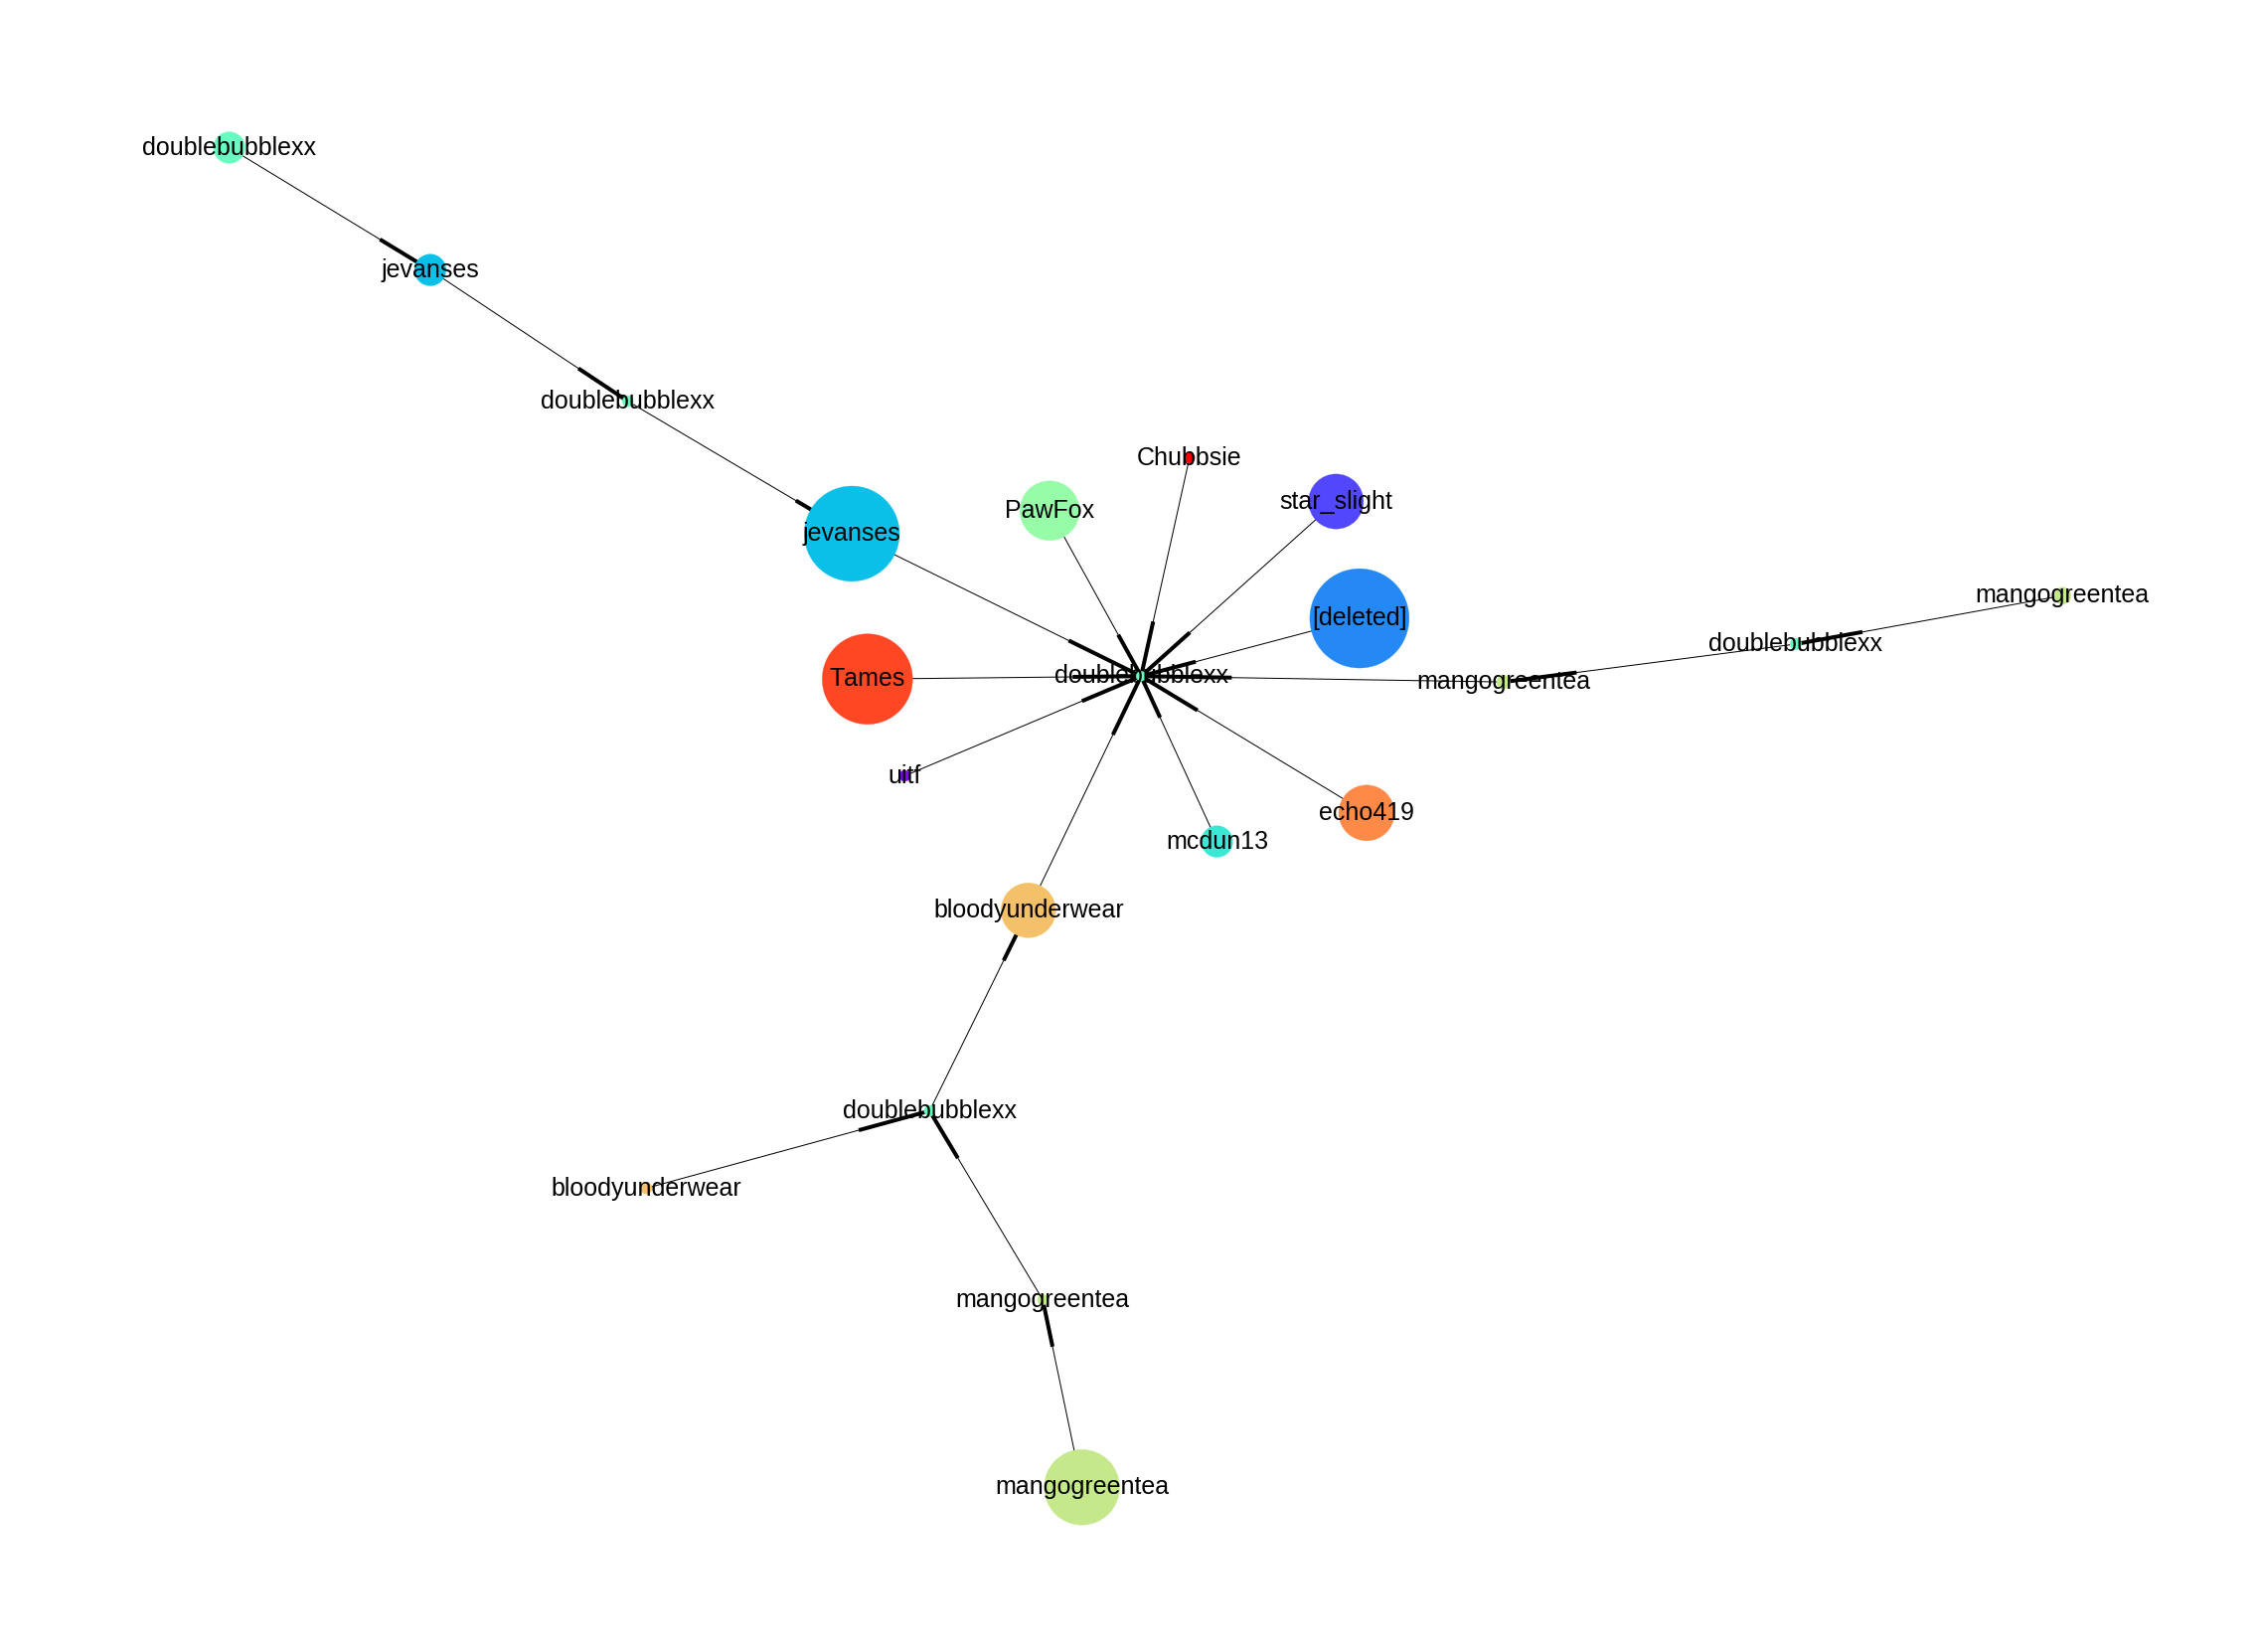
\includegraphics[width=0.45\textwidth, height = 5cm ]{ReplyGraphSW}
        \label{fig:rGraphSW}
    }
    \subfloat[]{
        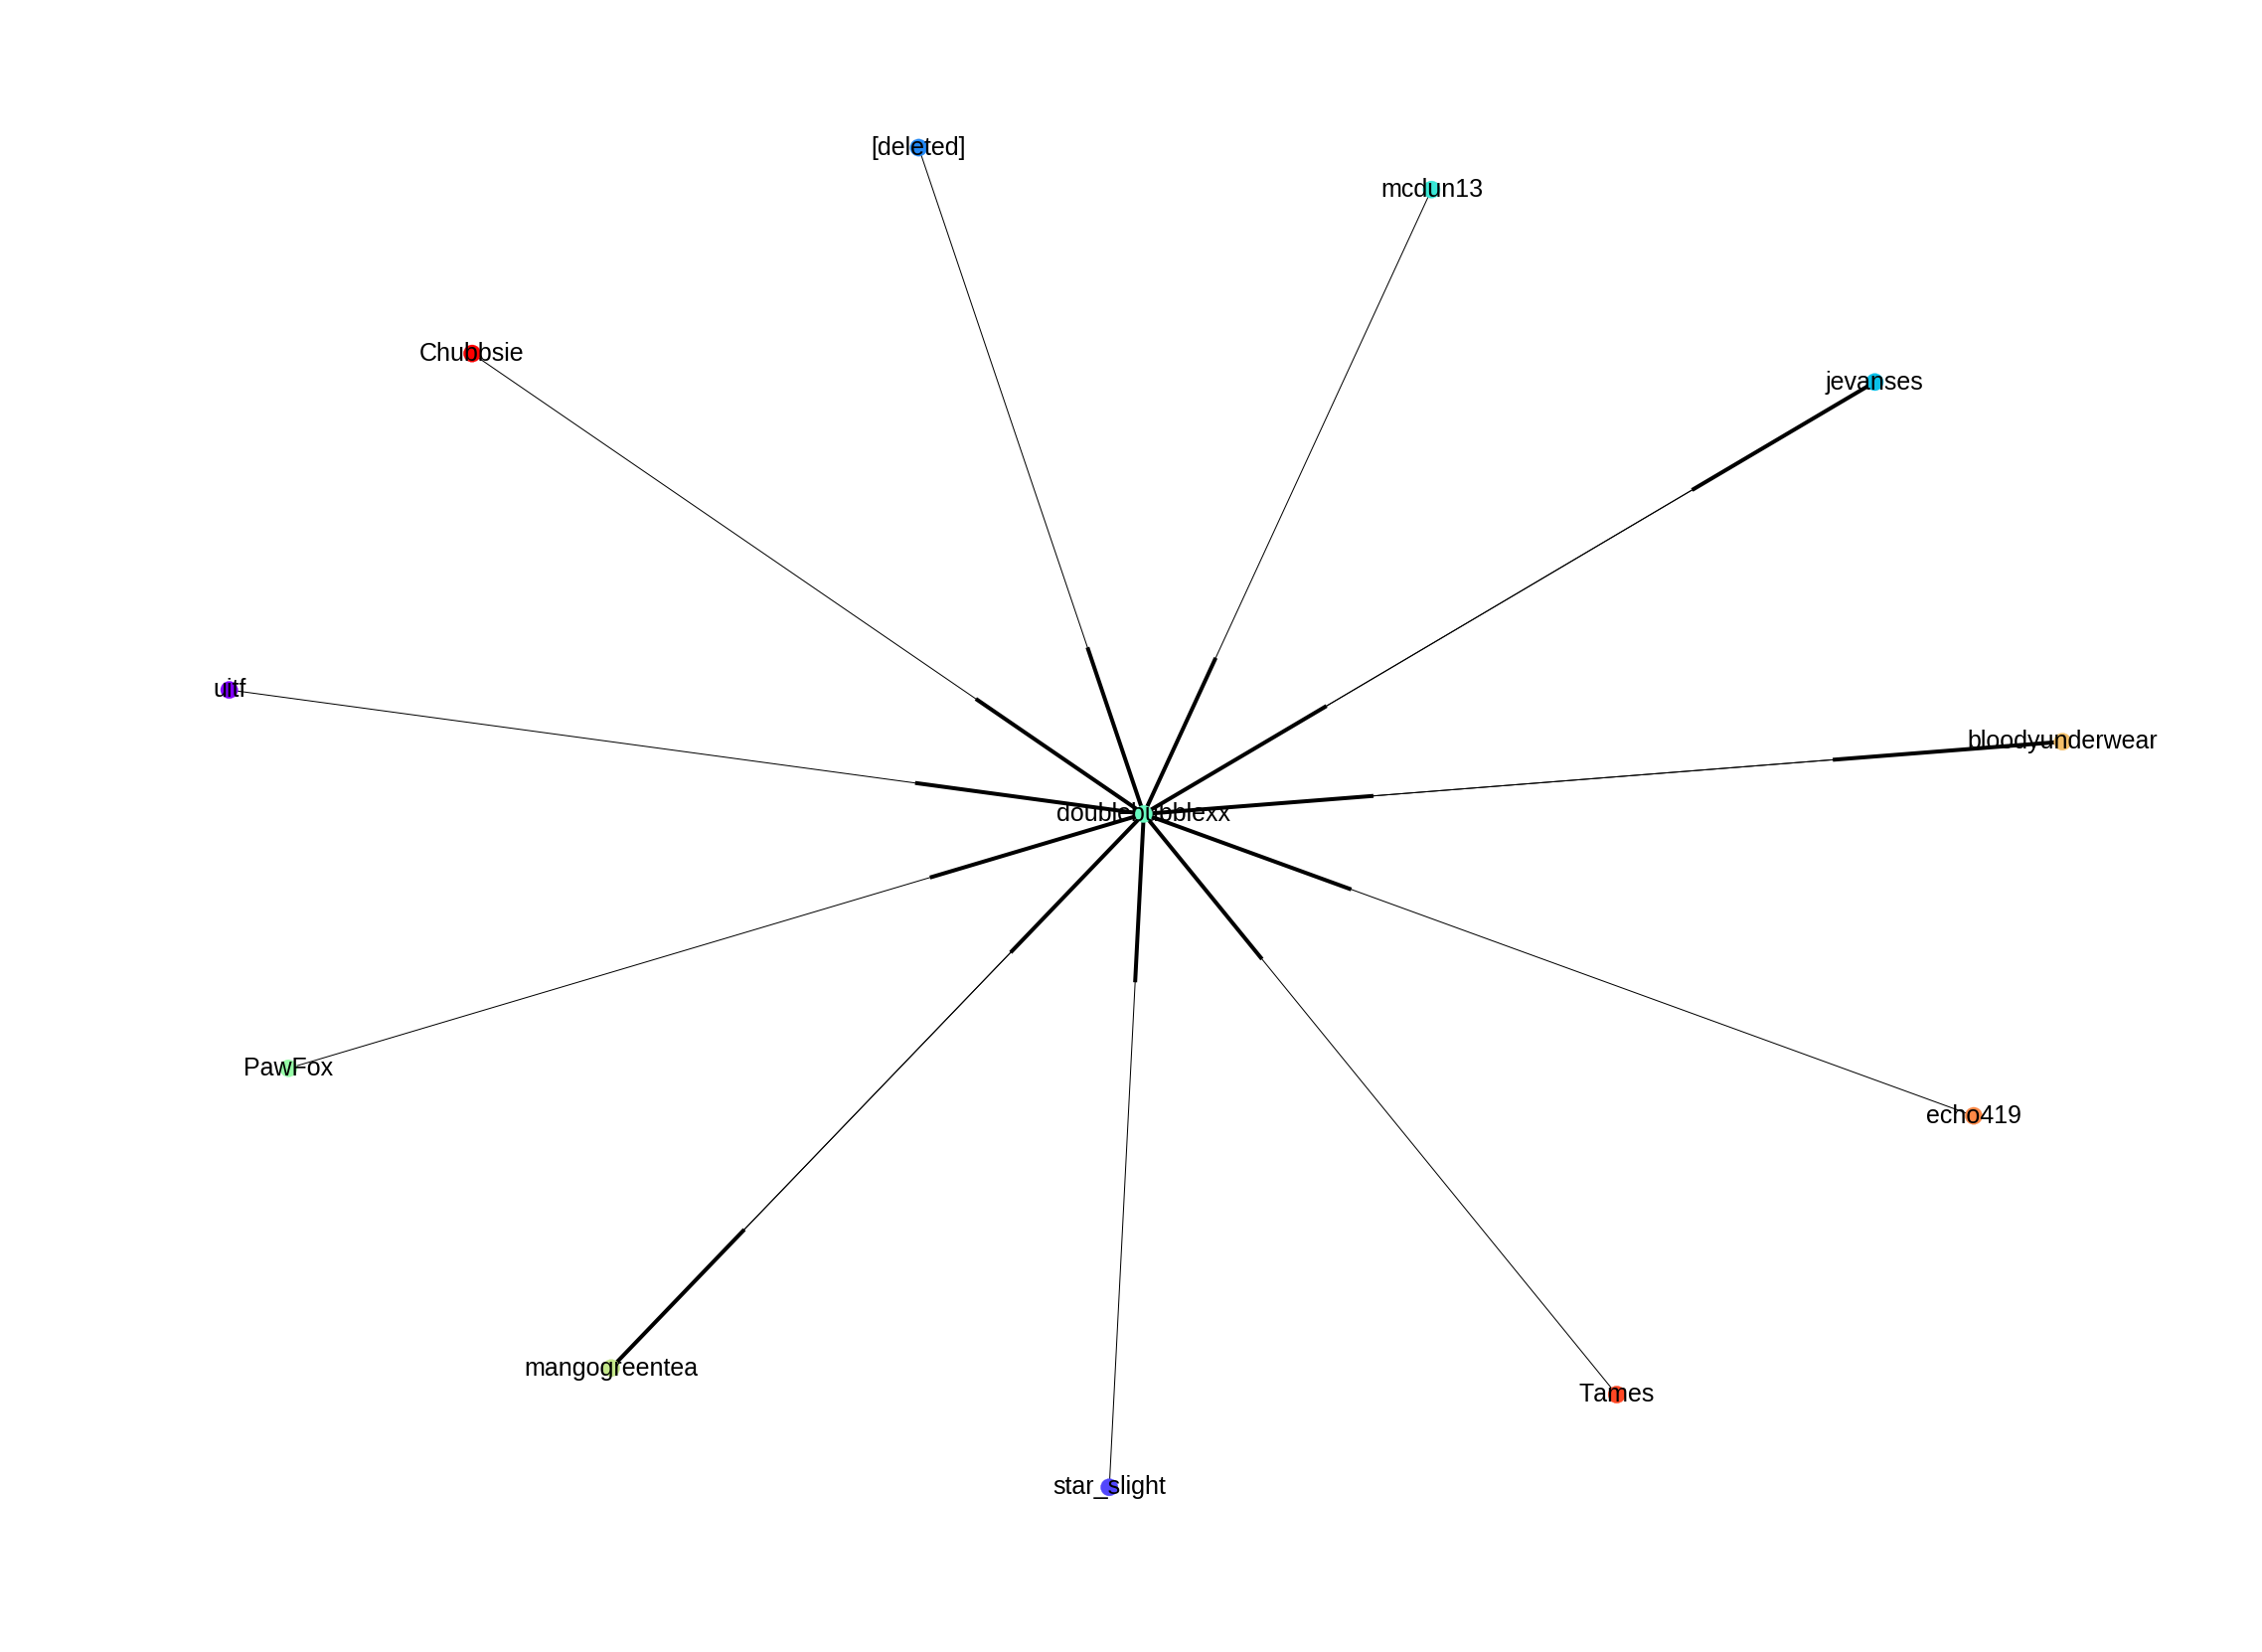
\includegraphics[width=0.45\linewidth, height = 5cm ]{UserGraphSW}
        \label{fig:uGraphSW}
    }
    
    
    \subfloat[]{
        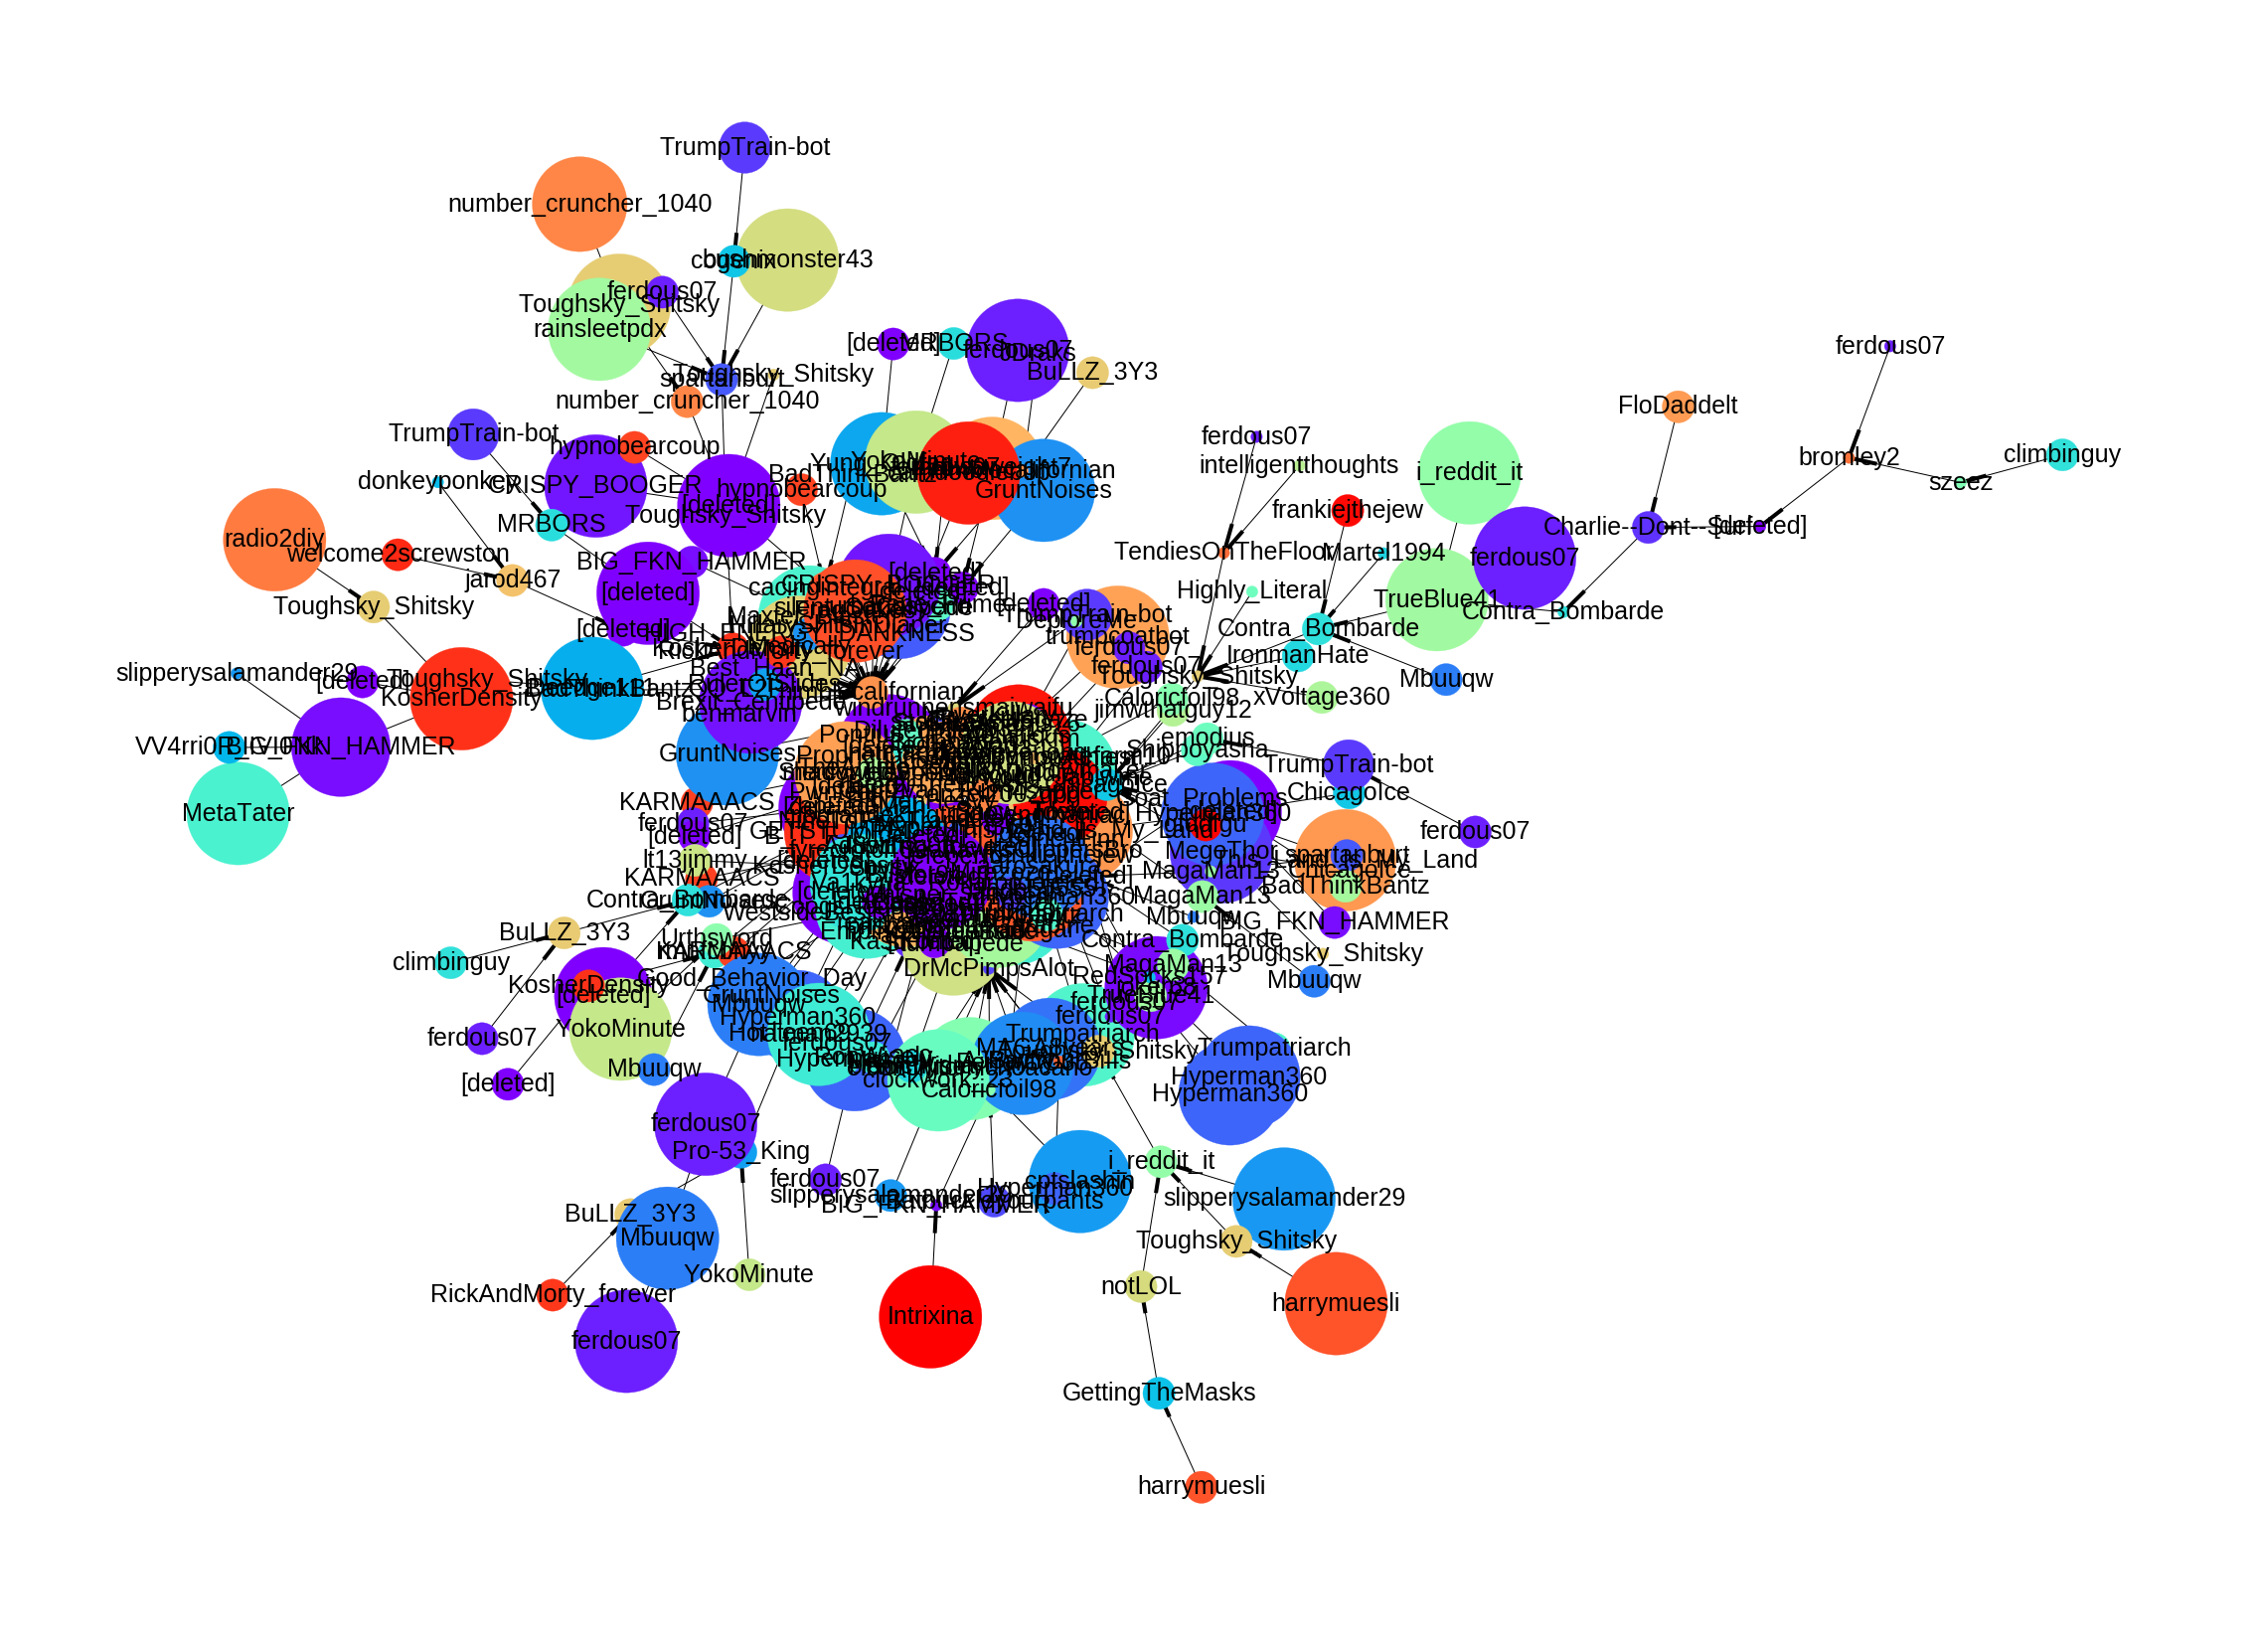
\includegraphics[width=0.45\linewidth, height = 5cm ]{ReplyGraphTD}
        \label{fig:rGraphFP}
    }
    \subfloat[]{
        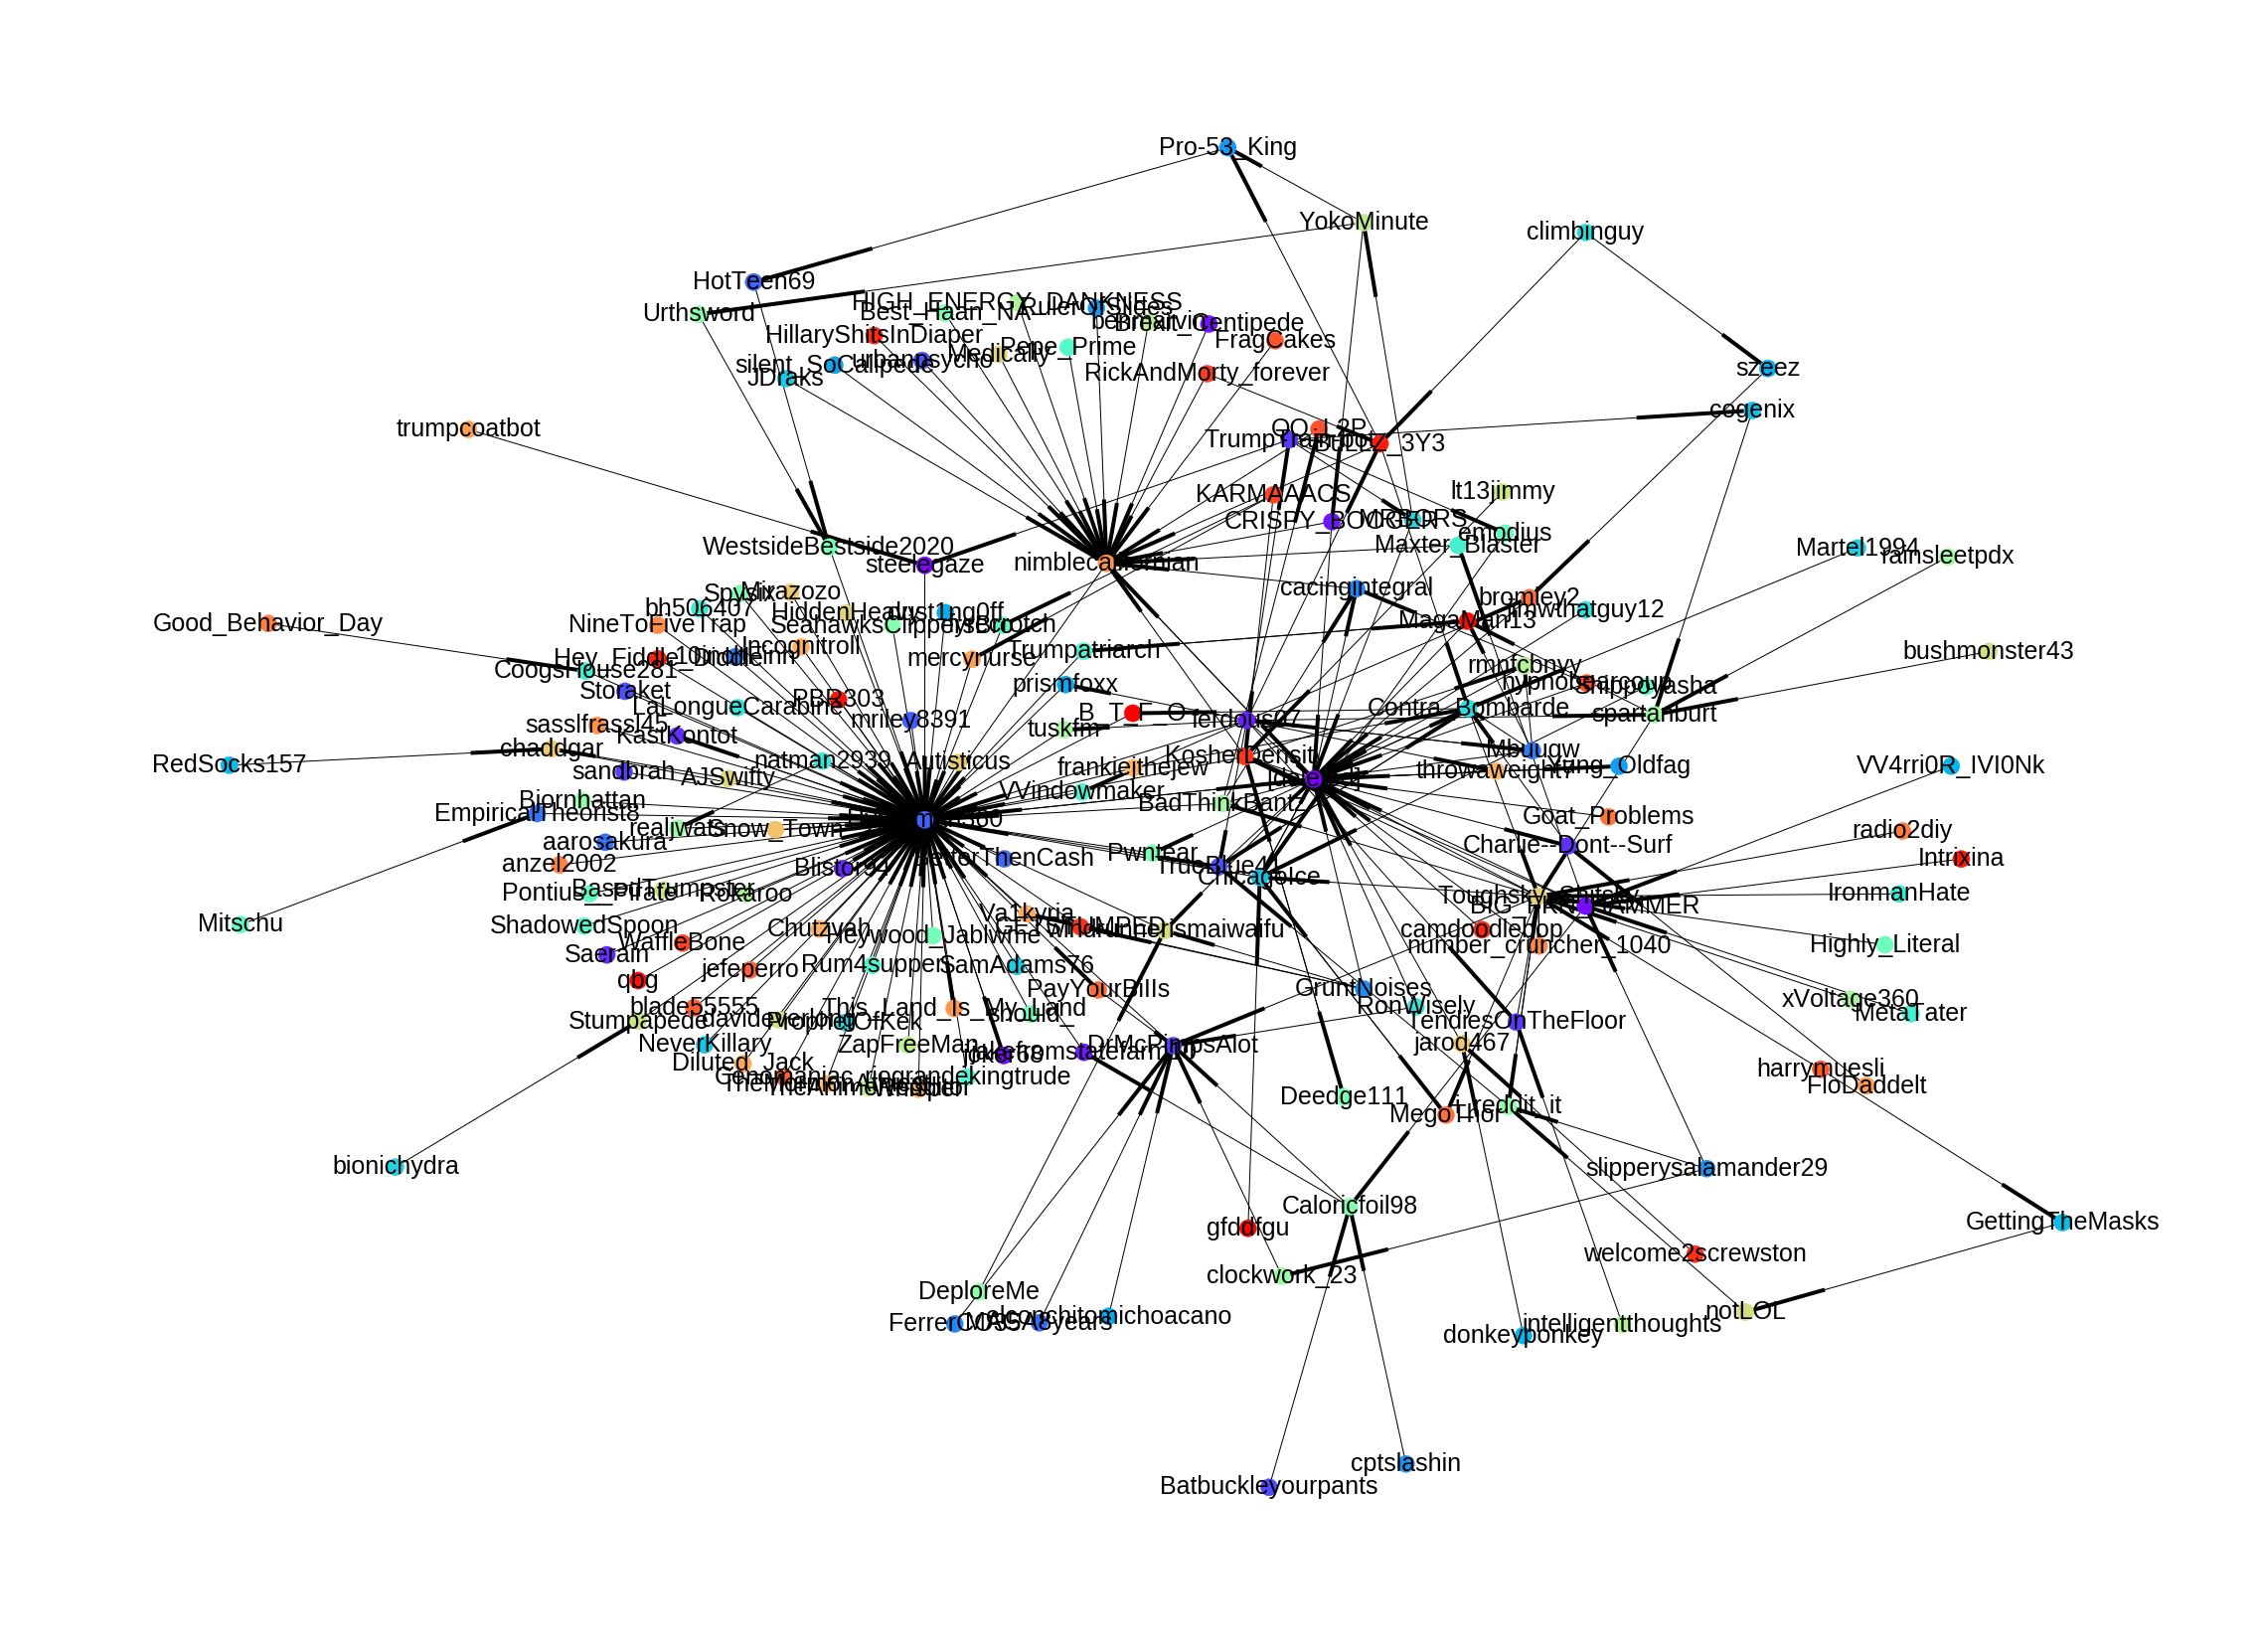
\includegraphics[width=0.45\linewidth, height = 5cm ]{UserGraphTD}
        \label{fig:uGraphFP}
    }
    \caption{ Example User graphs and their corresponding Reply graphs, Figure \ref{fig:rGraphSW} shows a random thread from the Suicide Watch sub-reddit along with the preserved structure of posts in the thread and \ref{fig:uGraphSW} shows the corresponding user graph that arises by capturing the user to user interaction in the thread from the reply graph. In comparison we have user graph Fig \ref{fig:uGraphFP} and its corresponding reply graph Fig \ref{fig:rGraphFP} from one of the Front page threads }
    \label{Fig:GraphExamples}
\end{figure*}

\subsubsection{Reply Graphs}
\label{Sec:Reply_graphs}
The first abstraction mimics directly the structure of conversation threads on Reddit. These abstractions are called Reply Graphs. We formulate a reply graph $R\{P,E,W\}$ as a thread of multi-layered posts in a thread in response to the root post $RP$ in the sub-reddit. Each graph $R$ consists of posts $P_i , P_j , i,j \in N$ , where N+1 is the total number of responses in the thread and edges $E_{ij}$ such that and edge $E_{ij}$ exists $iff$ post $P_i$ was in response to post $P_j$ in the hierarchy of responses.  The weight of the edge $E_{ij}$ is found by calculating the cosine similarity between semantic vector $V_i$ for post $P_i$ and the semantic vector $V_j$ of post $P_j$.  This abstraction works well in modeling the conversational nature of these forums.  For convenience of the reader, we present a couple of example pairs from SW and Frontpage baseline datasets in Figure \ref{Fig:GraphExamples}

\subsubsection{User interaction Graphs}
\label{Sec:Interaction_graphs}
In this method, we represent each thread as a directed graph $G\{V,E,W\}$ where $V$ is the set of all users participating in a particular thread and $E$ are the directed  edges which correspond to interactions between two users $V_i , V_j  \in V$. The weight of each directed edge $E_{ij}$ corresponds to the average of all the edge weights between $V_i , V_j  \in V$ in the corresponding reply graph $R\{P,E,W\}$ as described above. This means that each reply graph is then mapped to a User graphs where the nodes are users rather than posts. Another salient distinction between the two abstractions is that reply graphs resemble an n-ary tree and user graphs are directed cyclic graphs. 


\subsection{Network characteristics}
Figure \ref{fig:depthDist} shows the distribution of maximum depths across all Reply graphs for SW and Baseline subreddits. The SW threads depths have a median depth of 2 and mean of 4 compared to median depth of 2 for BL and a mean of 2.5. This shows that statistically the depths of Suicide watch and baseline graphs are quite similar.


\begin{figure}[!ht]
    \centering
    % \hspace*{-5mm}
    \subfloat[]{
        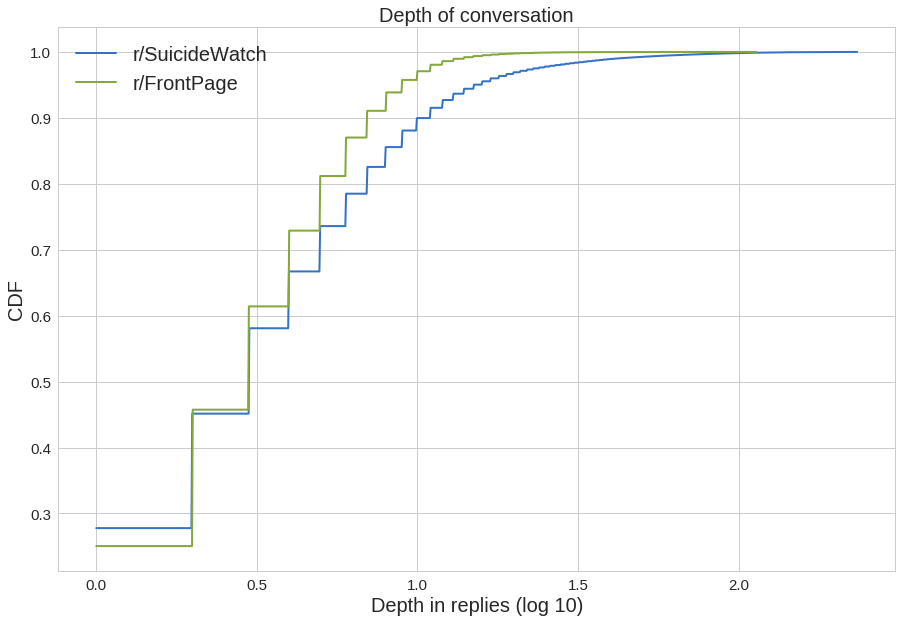
\includegraphics[width=0.4\textwidth]{ConvDepth.png}
        \label{fig:depthDist} }	
    \subfloat[]{
        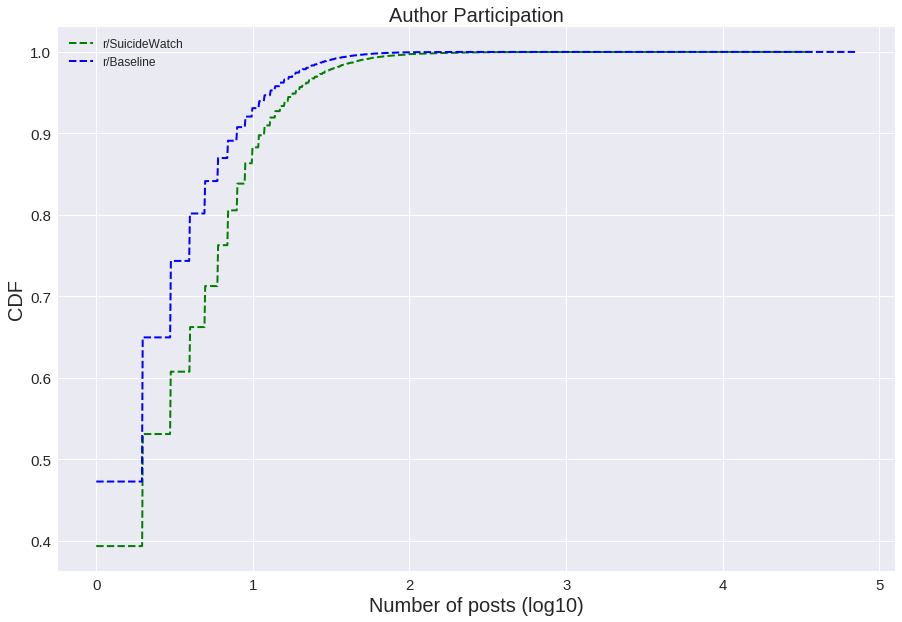
\includegraphics[width=0.4\linewidth ]{AuthorParticipation.png}
        \label{fig:uniqAuthors}
    }
    
    
    \subfloat[]{
        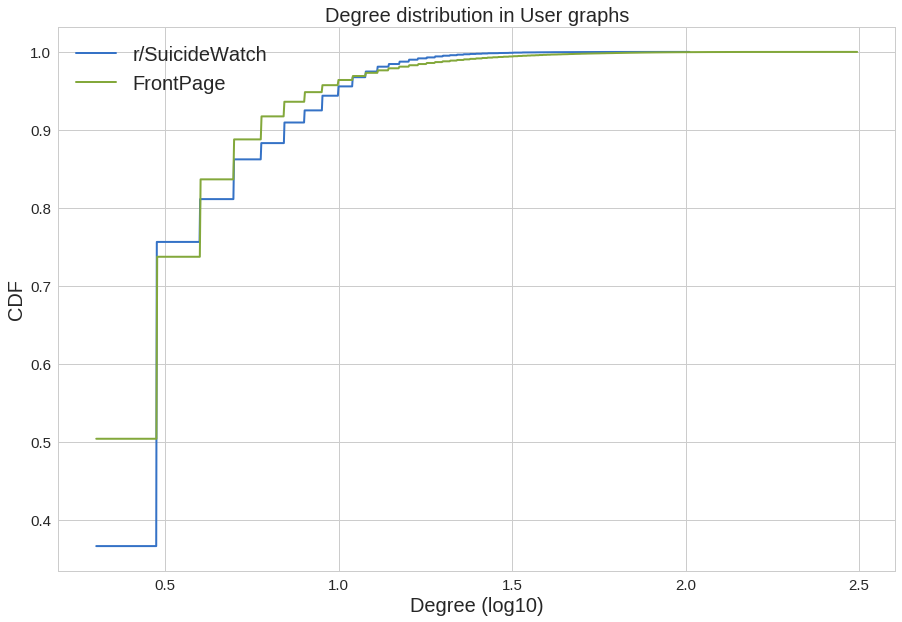
\includegraphics[width=0.4\textwidth ]{UserDegDist.png}
        \label{fig:degUgraph}
    }
    \subfloat[]{
        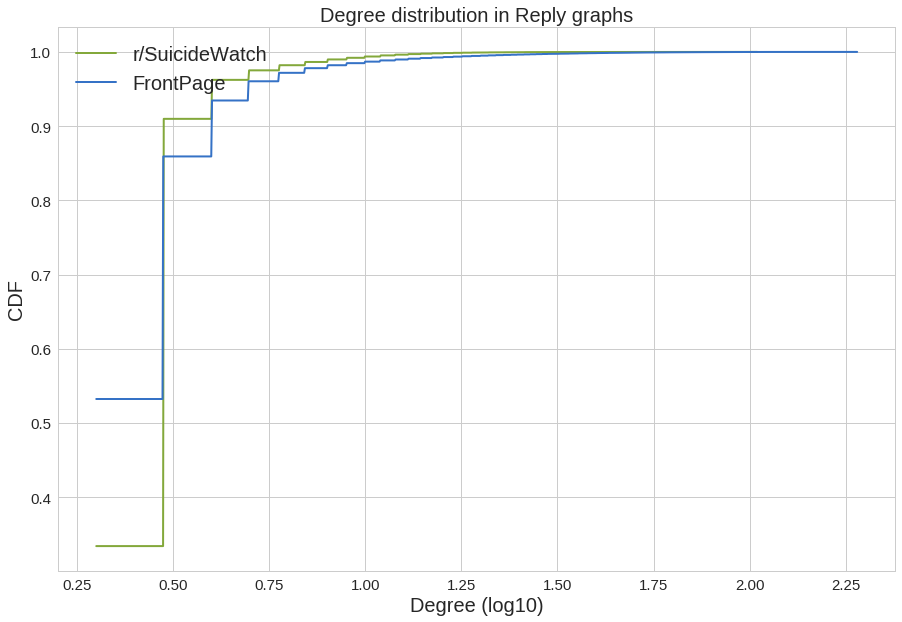
\includegraphics[width=0.4\linewidth]{ReplyDegDist.png}
        \label{fig:degRgraph}
    }
    \caption{\textsl{ Fig \ref{fig:depthDist} shows the distribution of maximum depths of Reply Graphs for Subreddit r/SuicideWatch and the baseline Frontpage conversations. Fig \ref{fig:uniqAuthors} shows the distribution of unique authors per thread in the two datasets. Fig \ref{fig:degRgraph} shows Distribution of degrees for Reply Graphs,  r/SuicideWatch and FrontPage. Fig \ref{fig:degUgraph} shows the degree distributions for the reply graphs}}
\end{figure}

\section{Metrics}

Once you are able to develop abstractions from the data, it becomes possible to develop metrics on these abstractions so as to derive insights about the mechanics of support. These metrics are then used to validate structural differences between supportive conversations and generic casual conversations from our baseline set, and come up with a theory for links between supportive conversations and the structure of the conversation, if we find any.



\subsubsection{Semantic Alignment}
\label{Sec:Semantic}
We use a popular word embedding method called \textit{Word2Vec} \cite{mikolov2013distributed} which learns representations of a set of words from a corpus of text, which in our case is the text from Suicide Watch and baseline fora. These representations can be used to extract text embedding vectors for each post which belong to a $N$ dimensional space $R^N$. These vectors are tested for their alignment using cosine distance in $R^N$, which from literature is shown to correspond to the semantic similarity in the textual space. This method is quite popular and used in community based question answering\cite{mihaylov2016semanticz}, Medical semantic similarity \cite{de2014medical} and other medical informatics applications\cite{zhu2017semantic}.
We first train two independent word2vec models on the Suicide watch and Front page post corpora. 
We then extract the word embedding vectors for each post using Doc2Vec\cite{le2014distributed}, which extends the word embeddings to represent a whole document or paragraph. We extract these embedding vectors for each post in $R^N$ for all the posts across the complete hierarchy of threads. We then quantify the edge weights of each interaction amongst the reply tree as the cosine distance between the response post and the hierarchically higher post, to which the responder has posted to. This captures the semantic alignment between the hierarchically adjacent responses. 
More formally, if user $V_i$ has responded with post $P_i$ to a post $P_j$ by user $V_j$, the edge weight of of edge $E_{ij}$ in the corresponding reply graph would be

$$ W_{ij} = \frac{V_i . V_j}{\|V_i\|_2 \|V_j\|_2} $$


This metric standardizes all edge weights between 0.0 and 1.0, 1.0 implying that the posts $P_i$ and $P_j$ are most aligned, and 0.0 implying the post have least semantic similarity. 
This metric abstracts out the content of the post, in terms of semantics which can then be used as edge weights in the graph abstractions.



\subsubsection{Centrality}
\label{Sec:Centrality}
For this metric we use the User Graphs. Node centrality is a metric that measures how central a node is in a network. It directly reflects the importance of the node when it comes to membership of the shortest connecting paths between all the nodes in the graph. More formally, we use betweenness centrality of a node which is defined as 
$$
g(v) = \sum_{s \neq v \neq t}\frac{\sigma_{st}(v)}{\sigma_{st}}
$$
where $\sigma_{st}(v)$ is the total number of shortest paths from node $s$ to node $t$ and $\sigma_{st}$ is the number of those paths that pass through $v$. To understand whether the thread starters ($OP$) have a special place in the network, we evaluate both centrality of the node corresponding to the $OP$, as well as median centrality across all the nodes in a user graph.

\subsubsection{Symmetrical users}
We define a symmetric user and a symmetric edges for user graphs. For a user $V_i$ in the user graph $G\{V,E,W\}$ as described in Section
, a symmetric user is a user who interacts with any user $V_o$ or the $OP$ and receives a response back from that user or the $OP$. We find the fraction 
$$
U_{sym}=\frac{\textit{total number of symmetric users }}{\textit{Total users in a thread}}
$$

\subsubsection{Urgency}
To understand the urgency in how Suicide watch subreddit users responds to the $OP$ and each other, compared to the baseline threads on the Frontpage, we calculate differences between the posting times between consecutive response messages in a reply graph. We then compute the median response times per thread, for posts in response to any $OP$ authored posts and in general across all other post responses. 

\subsubsection{Branching Factor}
\label{Sec:Branching}
Branching factor is a quantity that reflects the fan out of a conversation as it evolves.
To measure this phenomena, we use the reply graphs, which resemble a n-ary tree, to evaluate the branching factor. The branching factor is formally described as 
$$\tau = \frac{1}{|D|} \sum_{d \in D}^{} \frac{1}{|N_d|} \sum_{n\in N_d}^{} \textit{InDeg}(n)$$

%\subsubsection{Median semantic alignments}
%\label{Sec:Semantic_alignment}
%This metric quantifies the overall semantic alignment between response posts across a particular conversation thread. For any reply graph $R\{P,E,W\}$, we compute The median of all the edge weights calculated using the definition of semantic alignment 
%This metric quantifies the overall semantic alignment in a conversation. We also do the same calculation between responses to any post authored by the $OP$ to test whether responses to $OP$ demonstrate any special pattern of all alignment in supportive vs generic threads.



\section{Macroscopic analysis: at conversational level}

Through our analysis we find several discriminatory factors among Suicide watch conversations and generic front page conversation. We show that some of these factors are archetypal of suicide watch conversations such that they are over-expressed in suicide watch conversations to a very high degree. We also show that certain properties of these conversations can be backed by sociological theories of real life support conversations. 

\subsection{Peculiarity of threads of Support}
We begin by characterizing the two networked abstractions, namely Reply Graphs and Interaction graphs as described in Section \ref{Sec:Abstractions}. We do so by first comparing these two abstractions with a baseline control conversation threads using certain macroscopic network properties. 

\subsubsection{Responses to $OP$ are very urgent in supportive setting}
Understanding the inter message times can act as a good proxy for the urgency in a conversation. To understand how Suicide watch subreddit users responds to a $OP$ and other users as compared to other sub-reddit threads on the frontpage, we calculate differences between the posting times between consecutive messages in a reply graph. Figure \ref{fig:urgency} shows comparison using CDFs of inter-message response times for SW and FP threads. It can be seen that SW $OP$ are responded with the highest urgency amongst the 4, especially compared to either the $OP$ or any other users or sub-reddits. 

\begin{figure}[!ht]
    \centering
    % \hspace*{-5mm}
    \subfloat[]{
        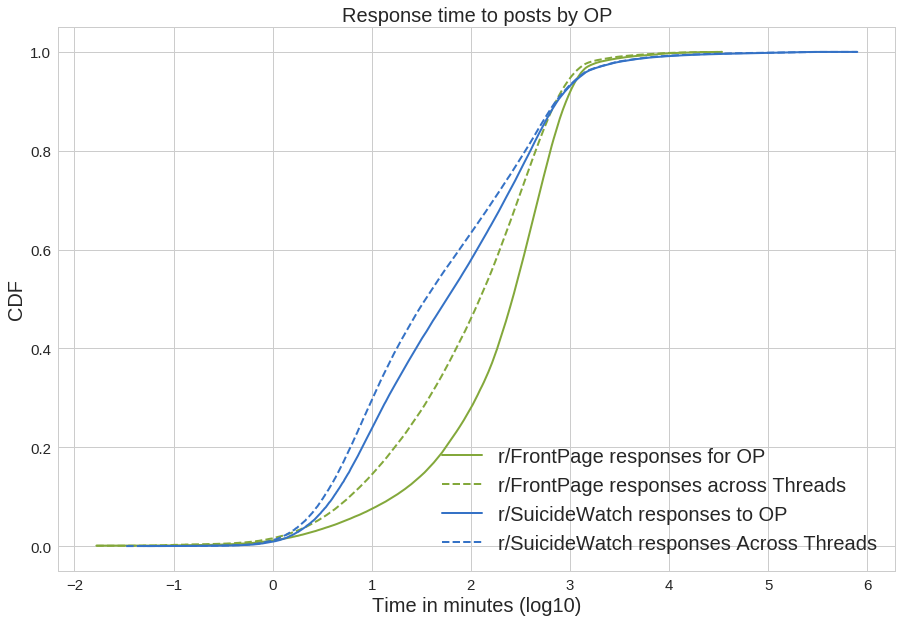
\includegraphics[width=0.4\textwidth ]{Urgency.png}
        \label{fig:urgency}
    }
    \subfloat[]{
        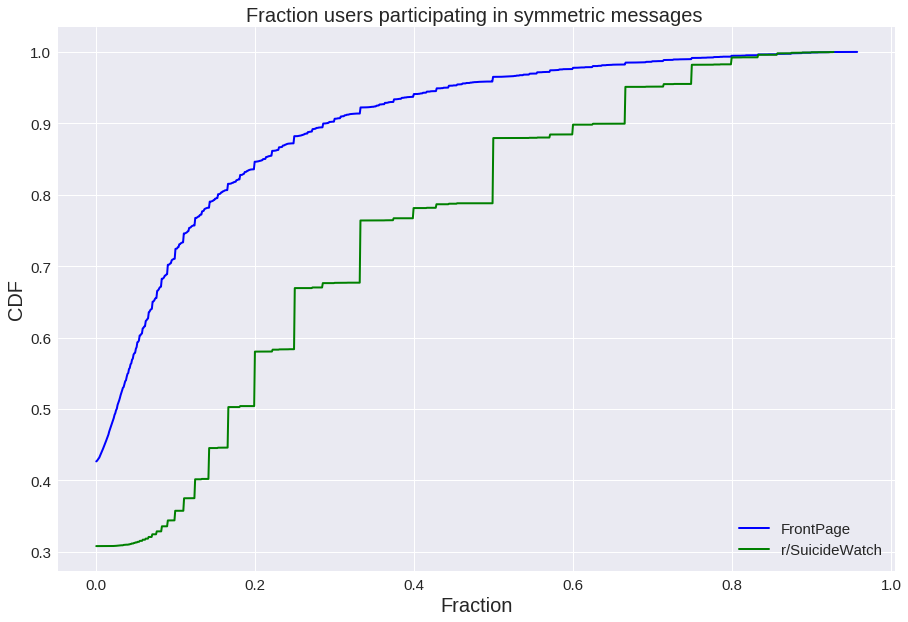
\includegraphics[width=0.4\linewidth ]{SymUsers.png}
        \label{fig:sym}
    }
    
    \subfloat[]{
        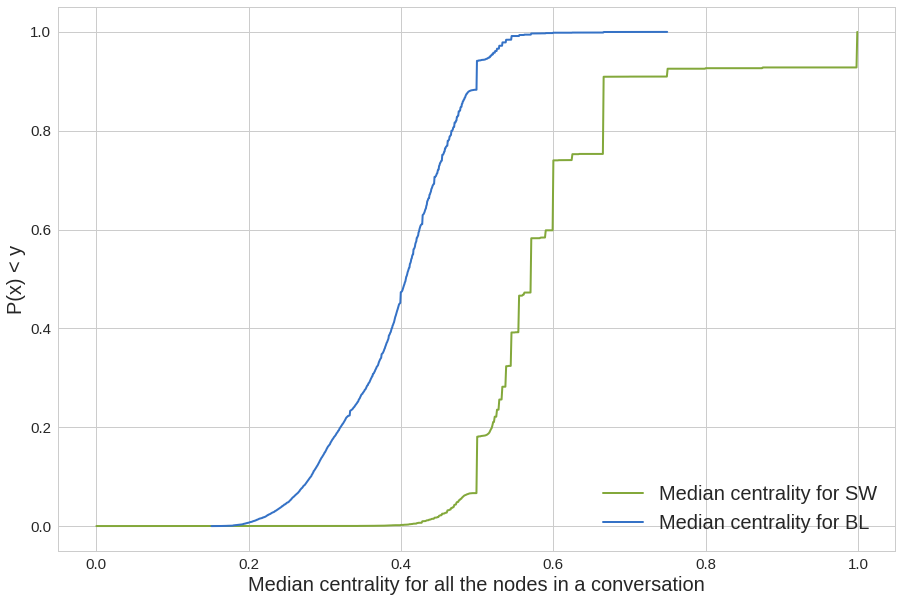
\includegraphics[width=0.4\linewidth ]{centrality.png}
        \label{fig:centrality}
    }
    \subfloat[]{
        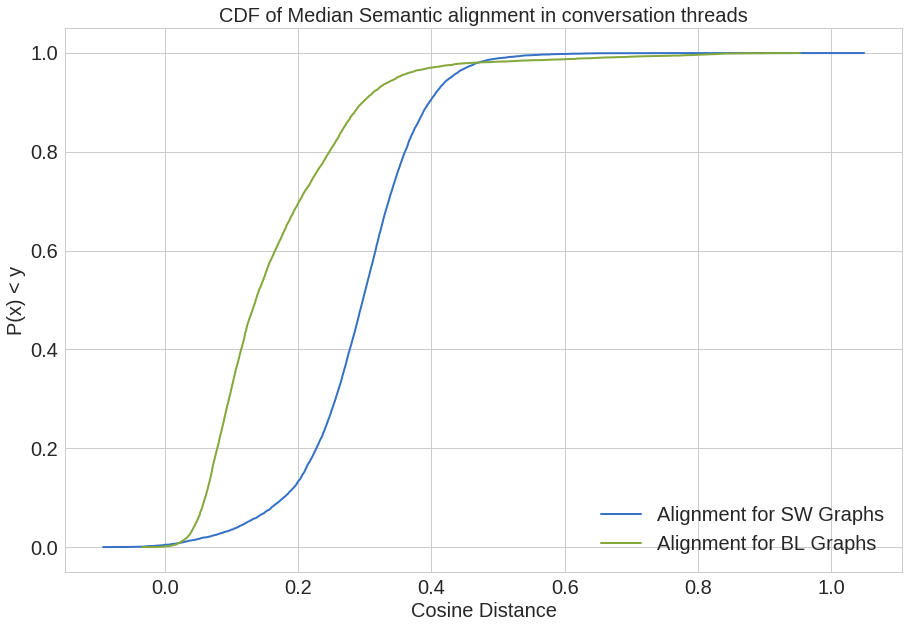
\includegraphics[width=0.4\linewidth ]{topicalAlignment.png}
        \label{fig:topical}
    }
    
    \subfloat[]{
        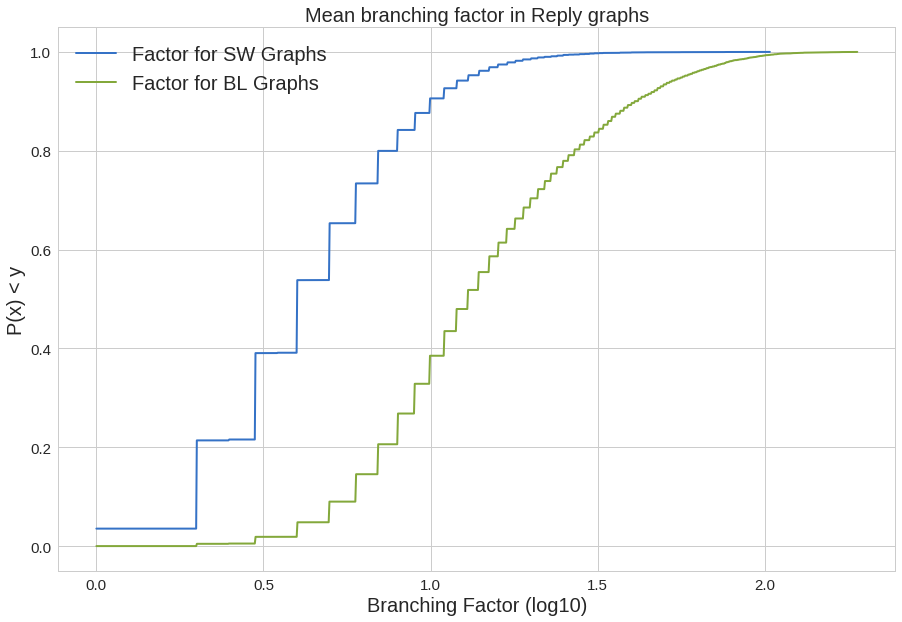
\includegraphics[width=0.4\linewidth ]{branchingFactor.png}
        \label{fig:branching}
    }
    
    
    \caption{Panel shows CDFs of different network metrics. Fig.\ref{fig:urgency} shows the response time distributions, Fig.\ref{fig:sym} shows symmetrically engaged users, Fig.\ref{fig:topical} shows topical similarities across posts and \ref{fig:branching} shows the branching factors of reply graphs. }
\end{figure}

\subsubsection{Interactions on suicide watch forums are statistically more symmetric}
Despite signs of urgency and engagement, we ask the question: what percentage of conversations happening on these subreddits are symmetric in nature ? 
For this The median value for $U_{sym}$ for SW is 20\% where as for AS is 0\%. This shows that SW subreddit engages is a lot more symmetric conversation that the baseline threads.
If we define a set of users who engage in symmetric activity with the $OP$ , it would be worth while to investigate how much of the total message activity on the thread is carried out by these set of symmetric users . To calculate this we find the fraction of messages on each thread written as part of this symmetric conversation. Figure \ref{fig:sym} shows the trend. It can be see that SW threads contain a higher prevalence of symmetric message exchanges compared to the baseline Frontpage threads. This shows a higher engagement from the $OP$s side when participating in a supportive conversations

\subsubsection{ $OP$ is the most central user in supportive conversations}
To understand how embedded is the $OP$ in a conversation thread, we compare the betweenness centralities of $OPs$ in the $SW$ dataset with the baseline $FP$ dataset. 
Betweenness centrality is a good proxy of understanding how closely linked is a node with the rest of the network. When we calculate this metric for the user graphs we see that Suicide watch $OP$s tend to have highest centralities compared to generic $FP$ threads moth in terms of $OP$ centrality as well as median centrality across all the users. The high centrality of $OP$s in $SW$ conversations implies a high level of embedded-ness as well as a $OP$ centric approach by other participants in the conversation. The Figure \ref{fig:centrality} shows the Empirical CDFs of centralities. 

\subsubsection{Supportive responses are semantically aligned, more so when they are in response to the $OP$}
We measure semantic alignment based on word embeddings of the source post and the reply post, at every edge of the reply graph. The detailed method of extracting semantic alignment along a post and its response is described in Section \ref{Sec:Semantic}. Extracting such similarity metrics, we compare the trend in response text being in semantic alignment with the parent text in the reply graphs. 


\subsubsection{Supportive conversations branch out considerably less compared to baseline}
Branching in a conversation thread could be either a sign of digression or a sign interestingness resulting in more people joining in. To measure this phenomena, we use the reply graphs, that mimic the conversation structure of the threads. By using the method described in Section \ref{Sec:Branching}, we found that Suicide watch threads, tend to branch less as compared to our baseline conversations. This implies that suicide watch threads tend to remain on topic and more often than not, a one-on-one conversation. Albeit many such dialogues may emerge with many participants, and hence that explains the high centrality of the $OP$ in all user interaction graphs. If the participants on a thread seldom interact amongst themselves, the corresponding interaction graph will have the $OP$ as the most central node.



\section{Mesoscopic analysis: Anchored triadic motifs. }
\label{Sec:motif}

\begin{figure*}[!ht]
    \centering
    % \hspace*{-5mm}
    \subfloat[]{
        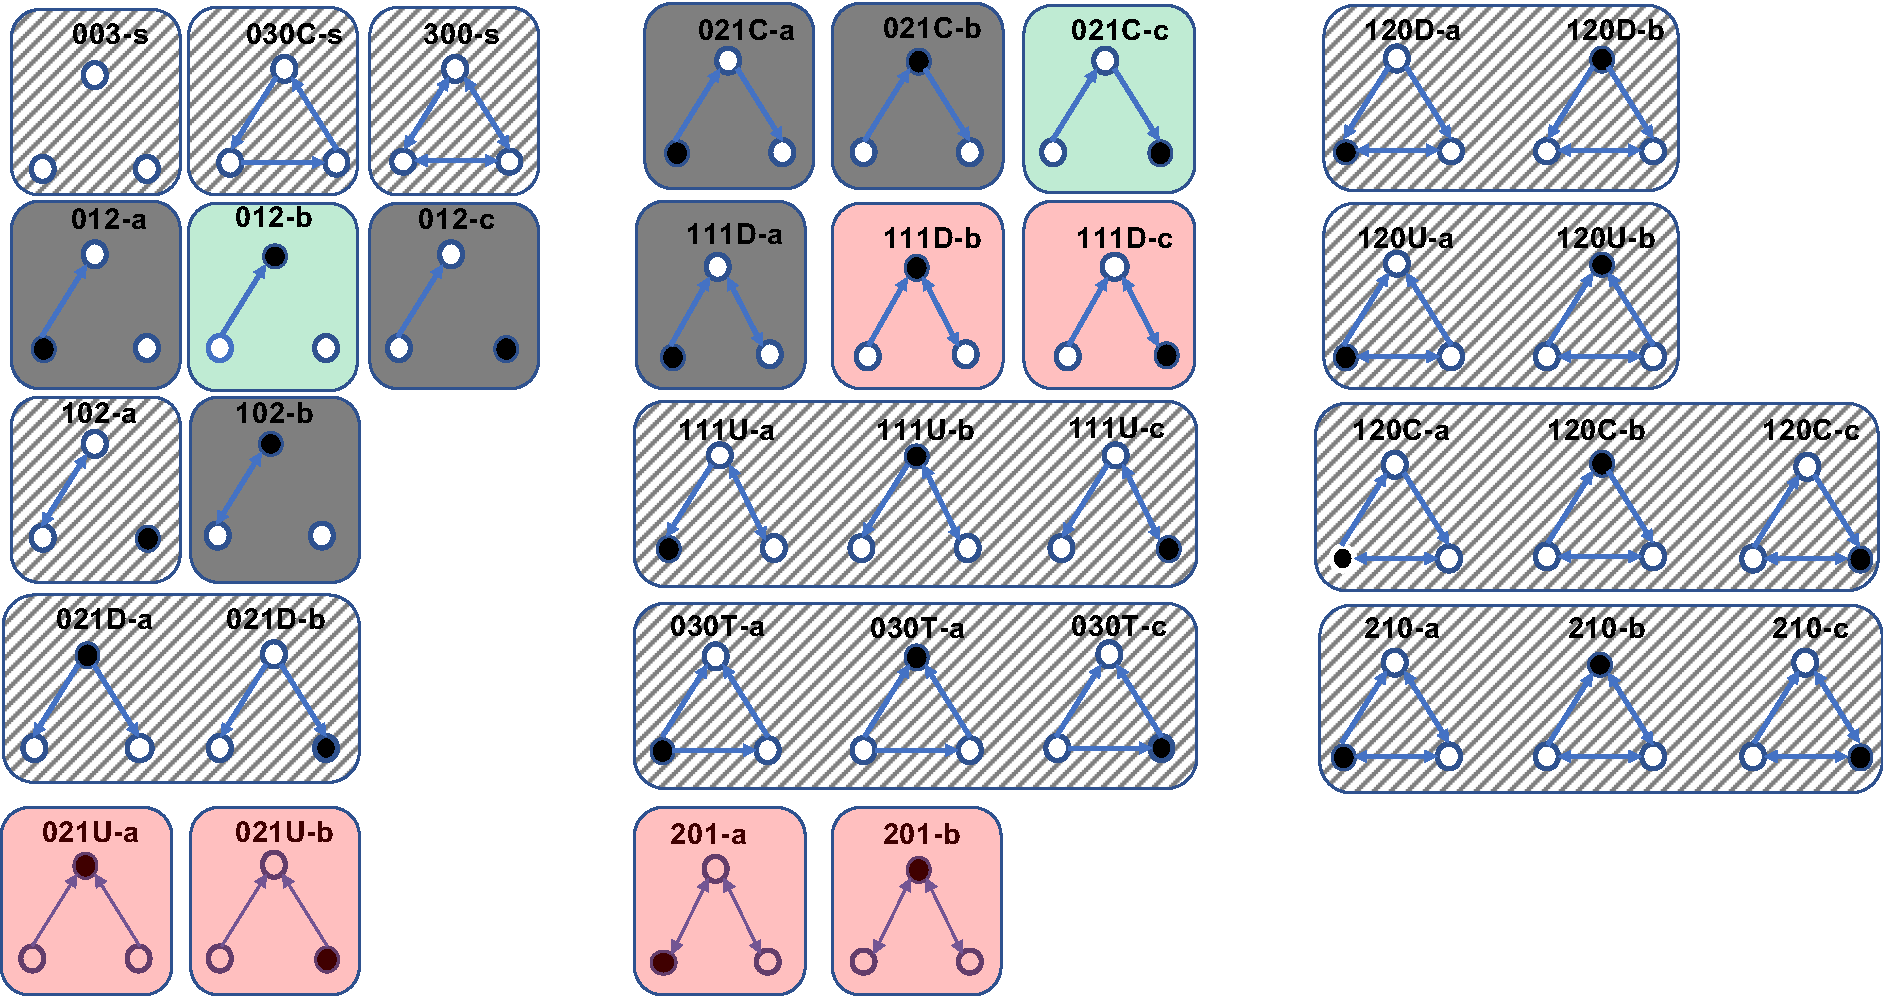
\includegraphics[width=\textwidth]{AnchoredMotifs_2.pdf}
        \label{fig:motifs}
    }
    
    \caption{ Figure \ref{fig:motifs} shows the 36 different types of Anchored Triadic motifs that are looked for in the user graph data. The motifs with \textbf{green boxes} are \textbf{over expressed in the baseline dataset} by significant amount. The motifs with \textbf{red boxes} are \textbf{over-expressed in the Suicide watch dataset} by significant amount. The motifs with \textbf{grey boxes} are present in significant numbers in both datasets, but neither over nor under expressed in any datasets based on their Z scores. The motifs in \textbf{grey hatched boxes} are very rare in both the baseline and suicide watch datasets, with less than 5 mean occurrences per graph per bin. 
    }
    \label{Fig:motifs}
\end{figure*}


Network motifs are local sub-networks between 2 or 3 nodes. Such local patterns are highly useful in quantifying local interactions and the resulting macro structure of the network\cite{milo2002network}. They have been used in a variety of applications and networks, from economics \cite{zhang2014dynamic} to cellular protein-protein interaction networks \cite{yeger2004network}. These local interaction patterns have been studied before, and have been fundamental in the study of social structural processes\cite{faust20077}. They help social scientists quantify the type of hierarchies in the social network\cite{davis1967clustering,davis1967structure}. 
But in the setup of a typical support community network like r/SuicideWatch, the conversation shows clear distinction between the users who respond to a call for help and the user/s who are asking for help. In the case of Reddit we define the former as the $OP$ who starts the conversation thread. For this reason, we changed the definition of the triadic motifs to accommodate the role of a node around which the motif is developed in the due course of the conversation. 
In conventional literature, the local interactions are measured in terms of census of 16 triadic motifs\cite{faust20077}, which cover all possible patterns of non-isomorphic graphs, or graphs which cannot be mapped or morphed into each other. In this method, there is no special treatment to any node, and positional parity of all nodes is treated equally. This means, role of a node in the conversation cannot be incorporated in this analysis. For this reason, we build on top of this methodology but by introducing anchors, or nodes with special importance. This is because, we would like to know how a graph evolves around the person in distress or the $OP$ in our case. A symmetric link with the $OP$ implies that the $OP$ is part of a to and fro communication, however a triad with a symmetric link between two non-$OP$ nodes implies that the conversation does not involve the $OP$. 
By fixing a role for a node in a motif, each of the 16 triadic motifs as seen and developed in the field\cite{faust20077, holland1977method}, can be unravelled into 36 sub-variants of these motifs by varying the anchored node, as seen in Fig \ref{Fig:motifs}. Each sub-variant is different from the other from the perspective of the anchored node. The resulting motifs to measure grow from 16 to 36, since some anchored motifs are iso-morphic, which means they look identical to some other motif from the perspective of the anchor. These motifs are then counted using custom tweaked census methods based on Bataglej et.al's work\cite{Batagelj2001}.
Each motif as seen in Figure \ref{fig:motifs} is named using a particular recipe. The first three letters, follow a M-A-N pattern which signifies the number of "\textbf{M}utual" , "\textbf{A}symmetric" or "\textbf{N}ull" edges present in that particular triad. E.g. the motif 030 has 0-Mutual(bi-directional), 3-Asymmetric(unidirectional) and 0-Null(disconnected) edges. There are some motifs with an added letter modifier attached, to signify the flow of information in the triad. The naming is done in accordance with Holland et. al's work\cite{doi:10.1177/104649647100200201}.


To methodically understand the over or under expression of these anchored triadic motifs in the suicide watch community, we use the user interaction graphs for the Front page baseline posts as a control group. We analyse 10,000 user interaction graphs each for the baseline and the suicide watch datasets.
We progressively select graphs with variable sizes i.e. number of users present in the interaction graphs. We do so by binning each dataset in ranges of graph sizes in increments of 5 nodes per bin. The resulting graphs would fall in the following 7 bins, with increasing number of nodes present : 1 - 5 , 6 - 10 , 11 - 15 , 16 - 20 , 21 - 25, 26 - 30, 31 - 35 and 36 - 40. We stop sampling above 40 nodes per graph, as the population of conversations that contain more than 40 unique users participating is extremely scarce for both the datasets.
We then do the census for the 36 unrolled motifs for each of these bins, for both the datasets. 
Once the census is done, we calculate $Z_{scores}$ for the Suicide watch conversations, using Baseline conversations as the null model, to understand over or under expressions of certain motifs. 
For any given bin $B_I$, let there be $k$ baseline graphs that fall in that particular bin noted by $G_{BL}$ , and let there be $n$ suicide watch graphs falling in the same bin signified by $G_{SW}$. For such a setup, let $M_{BL}$ signify a vector of $k$ elements, where each element is the total number of occurrences of particular motif $m$ in each graph from the set $G_{BL}$. With this sample of graphs as the null model, the mean would be $\mu_{null} = \frac{1}{k}\sum_{m_i \in M_{BL}}^{}m_i$ , where $m_i$ is the count of motif $m$ in the $i^{th}$ graph in  $G_{BL}$. The standard deviation $\sigma_{null}$ is $std(M_{BL})$
Once we have the null model parameters for the baseline graphs for a particular bin, we calculate $Z_{scores}$ for all the graphs from suicide watch samples $G_{SW}$ from the same corresponding bin as random variable $Z$ where the $i^{th}$ element is the $Z_{score}$ for graph $i$ in $G_{SW}$. The score is calculated by the following formula 

$$ Z_i = \frac{m_i^{sw} - \mu_{null}}{\sigma_{null}} $$ 

where $m_i^{sw}$ is the total number of occurrences for motif $m$ in the $i^{th}$ graph for the suicide watch samples. We then plot the mean of random variable $Z$ and the standard error in $Z$ to understand the over/under expression trends.


\subsection{Patterns in local interactions}
It is often useful to express large interaction graphs, as the sum of local interactions between two or three nodes at a time. This method is quite prevalent in the Social sciences, for studying social structures by looking at local interaction between agents\cite{faust20077}. Such analysis is quite useful in expressing local structures in the graphs and has been used in several network analysis works\cite{wang2014triadic,shizuka2015network}.
For this reason we conduct a census of the 36 Anchored triadic motifs (described in Section \ref{Sec:motif}) across all the selected graphs. From the amount of over or under expression of the network motifs, researchers have made inferences about the nature of local interaction. They do so by comparing the amount of density of each triad in a real network as against the expected quantity in a null model based on the number of edges\cite{faust20077}. 
We perform binning of user graphs as described before in Section \ref{Sec:motif}, and perform over or under expression analysis in comparison with the baseline null model, using Z-scores of the motif occurrences.



\begin{figure*}[!ht]
    \centering
    
    \subfloat[]{
        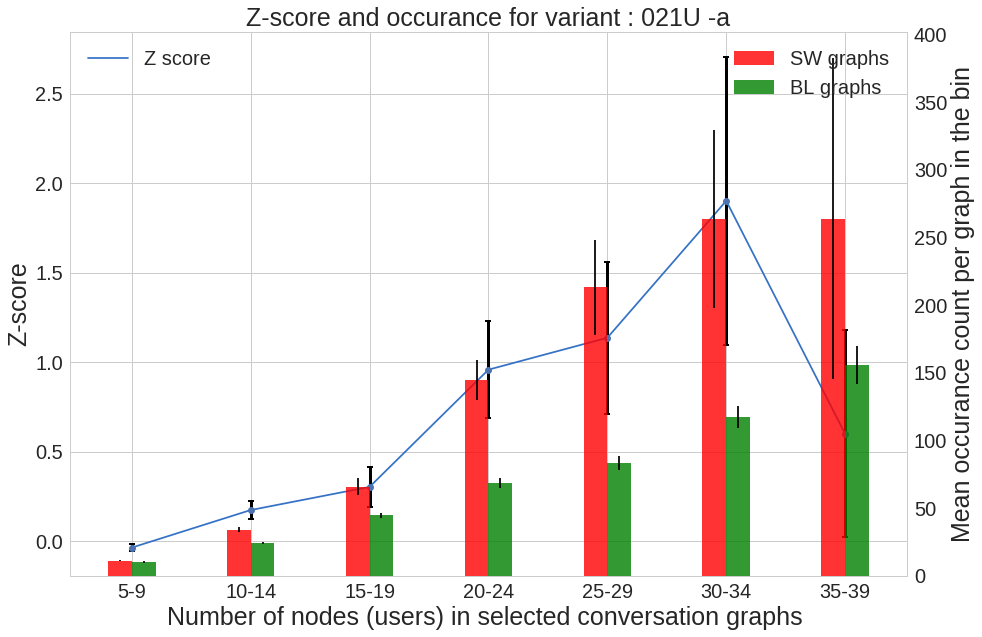
\includegraphics[width=0.33\linewidth ]{021U-a_SW.png}
        \label{fig:021U-a}
    }
    \subfloat[]{
        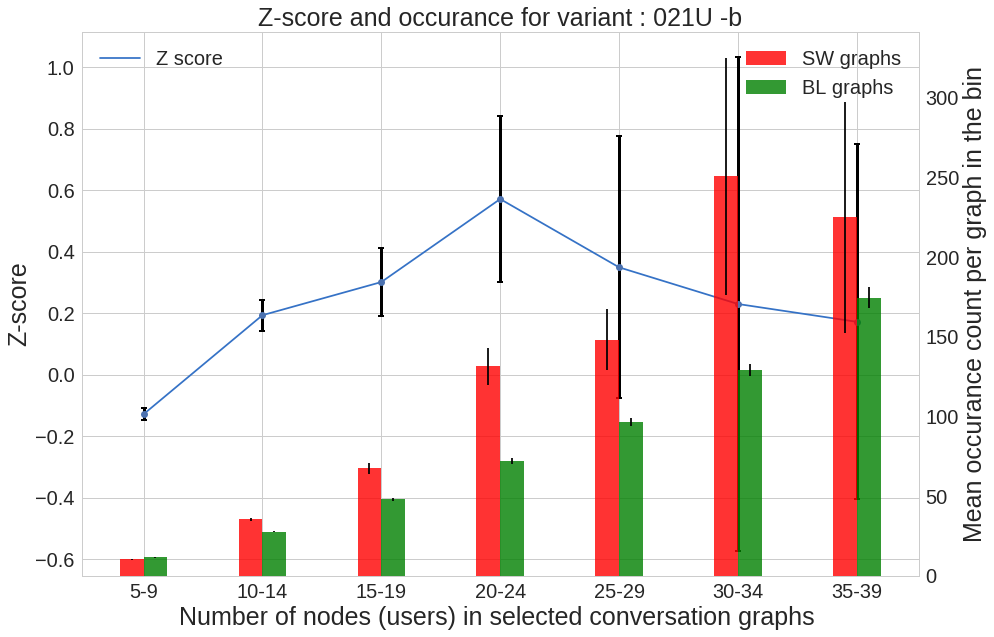
\includegraphics[width=0.33\linewidth ]{021U-b_SW.png}
        \label{fig:021U-b}
    }
    \subfloat[]{
        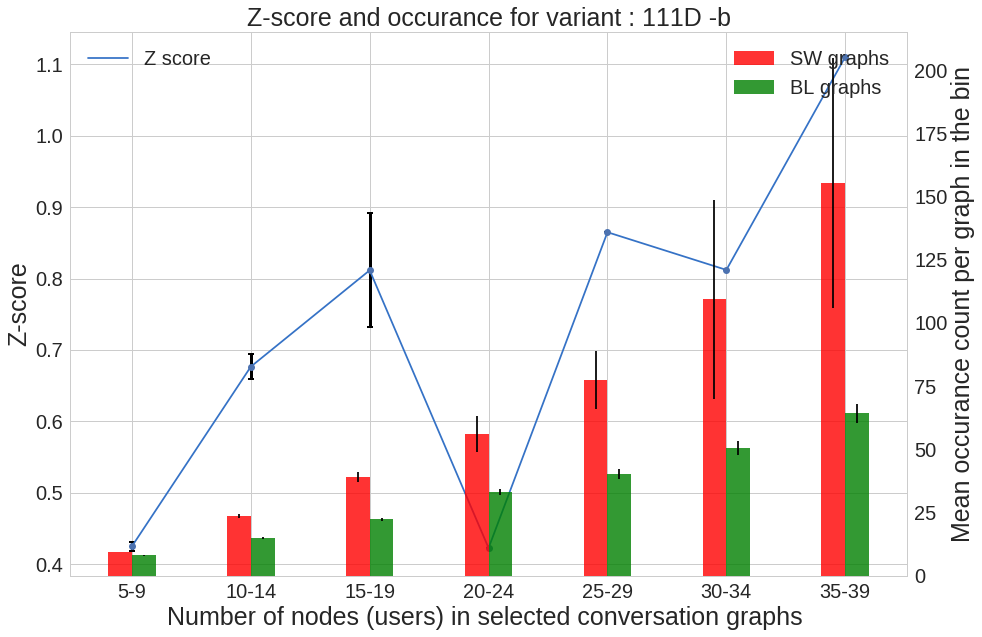
\includegraphics[width=0.33\linewidth ]{111D-b_SW.png}
        \label{fig:111D-b}
    }
    
    \subfloat[]{
        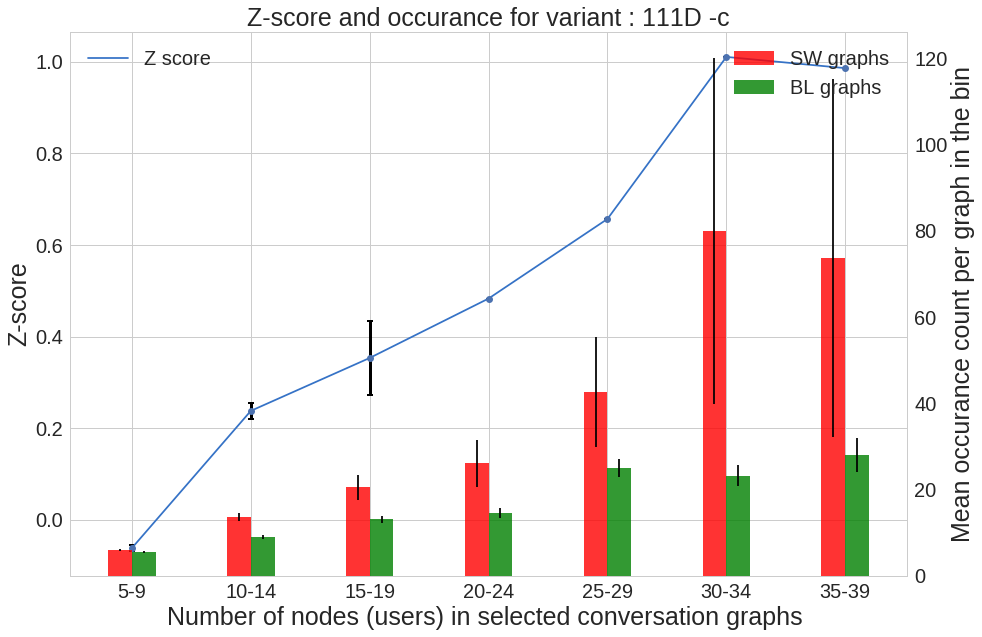
\includegraphics[width=0.33\linewidth ]{111D-c_SW.png}
        \label{fig:111D-c}
    }    
    \subfloat[]{
        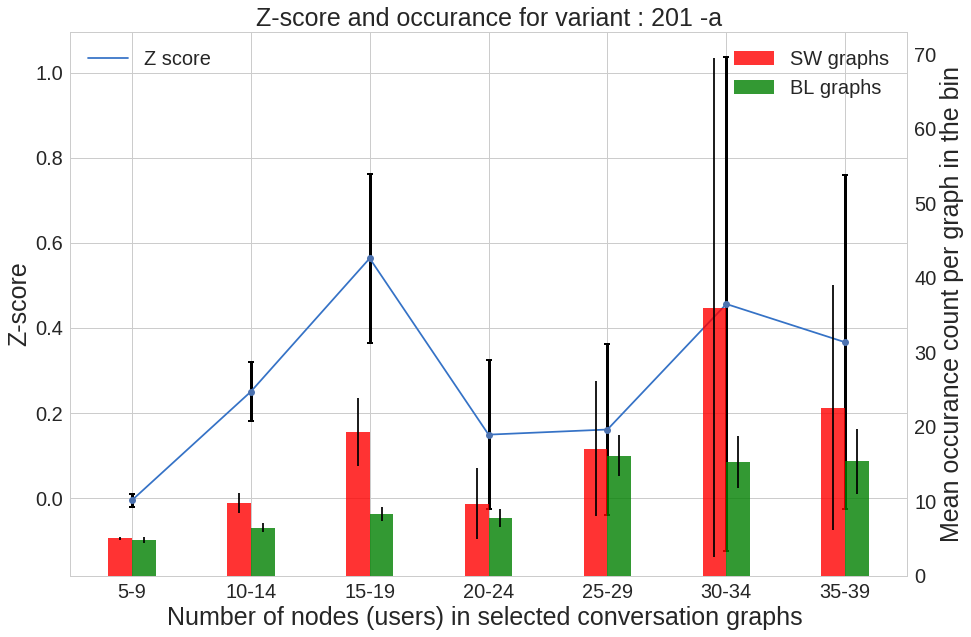
\includegraphics[width=0.33\linewidth ]{201-a_SW.png}
        \label{fig:201-a}
    }
    \subfloat[]{
        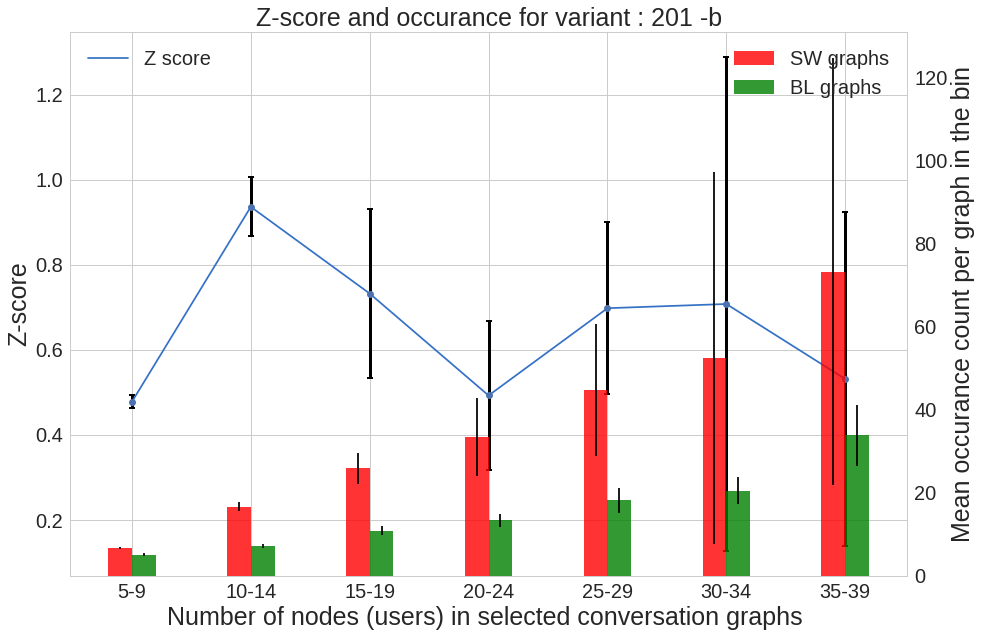
\includegraphics[width=0.33\linewidth ]{201-b_SW.png}
        \label{fig:201-b}
    }
    
    \subfloat[]{
        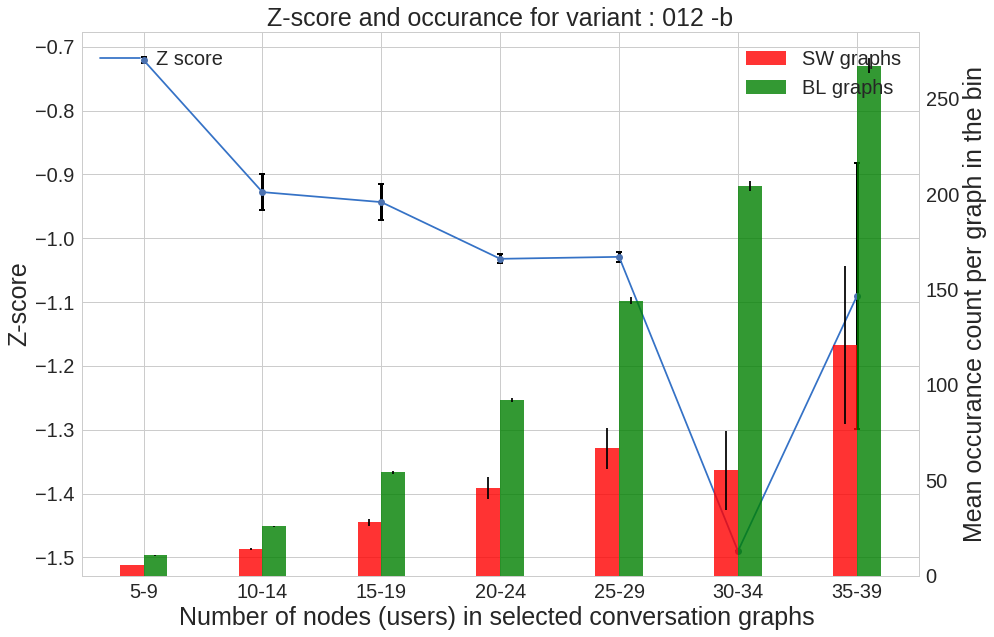
\includegraphics[width=0.33\linewidth ]{012-b_BL.png}
        \label{fig:012-b}
    }	
    \subfloat[]{
        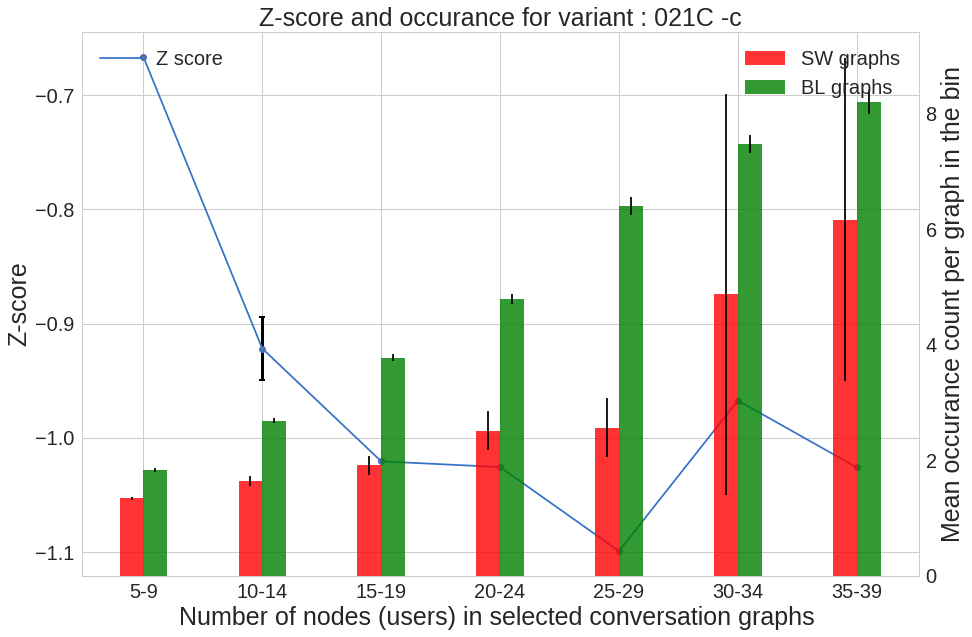
\includegraphics[width=0.33\linewidth ]{021C-c_BL.png}
        \label{fig:021C-c}
    }
    \caption{This panel shows the Z-scores of the abundant and over expressed Anchored motifs found in both datasets. There are variants which are over expressed in Suicide watch (Like figures \ref{fig:021U-a},\ref{fig:021U-b},\ref{fig:111D-b},\ref{fig:111D-c}, \ref{fig:201-a},\ref{fig:201-b}), which form the top six plots. The bottom 2 plots show motifs which are over expressed in the Baseline over Suicide watch, as their Z-scores are negative.  Figure \ref{fig:012-b} and Figure \ref{fig:021C-c}.
    }
    \label{Fig:motif_expressed}
\end{figure*}


\begin{figure*}[!ht]
    \centering
    
    \subfloat[]{
        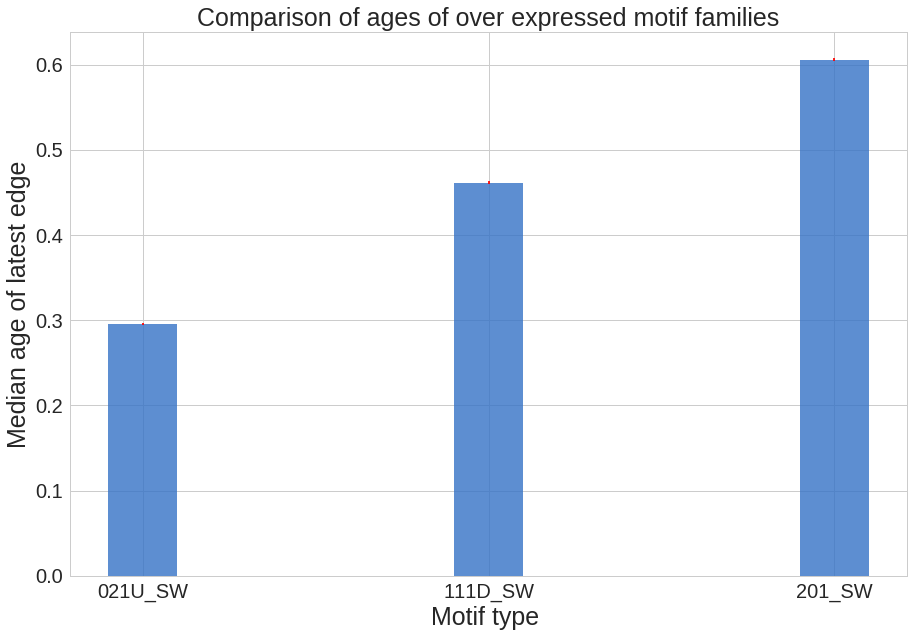
\includegraphics[width=0.4\linewidth]{motifLifetimes}
        \label{fig:motifDist}
    }

    \subfloat[]{
        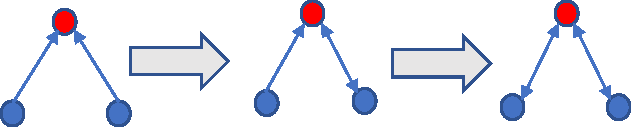
\includegraphics[width=0.4\linewidth]{Conversation_progress}
        \label{fig:convProgress}
    }
     \caption{\textsl{ Figure ~\ref{fig:motifDist} shows the plot for mean motif life times as a fraction of the entire thread life. The lifetime is measured as the time at which the latest edge of motif is formed. The Figure ~\ref{fig:convProgress} shows a toy example of what sort of dialogue exchange could lead to the motif lifetime distributions seen in Figure~\ref{fig:motifDist}}}
     
\end{figure*}
     



We find that anchored motif variants \textbf{021U-a, 021U-b, 111D-b, 111D-c, 201-a and 201-b} are significantly over expressed in suicide watch conversations across all sizes of graphs as seen from figures \ref{fig:021U-a},\ref{fig:021U-b},\ref{fig:111D-b},\ref{fig:111D-c}, \ref{fig:201-a},\ref{fig:201-b}. Similarly anchored motif variants \textbf{012-b and 021C-c} are significantly over expressed in the null model(baseline) graphs across all sizes.

From previous studies on triadic structure, it was inferred that transitive triads are naturally more common than expected in social structures of human social networks. Interestingly, our analysis shows that transitive triads are rarer in Suicide watch, as against the baseline conversations. But in the defence of previous studies, the networks we study are of human conversations and not of human social ties. Also these conversations are happening with an intent of providing support, which makes one user (the one in distress) the centre of conversation. These conversational preferences make the macro and meso level structural signatures peculiar.

\section{Conclusions and Outlook}

These patterns in local interactions indicate that conversations in suicide watch tend to be more $OP$ centric, with non-transitive dialogues between users who respond to a call for help. More so, the $OP$ tends to be highly central in the conversation as well as part of several mutual interactions. These behaviours are highly particular to r/Suicidewatch when compared with the baseline conversations. Further investigation of local structures in graphs show that there is a radically different way the conversation graphs evolve. The difference is not only between supportive conversation graphs and generic conversations, but also overall in supportive conversations and any social graphs. 
Several studies have looked at the social-tie structures and shown certain triadic motifs to be important in maintaining social hierarchy~\cite{shizuka2015network,shizuka2012social,holland1976local,doi:10.1177/104649647100200201}. But these expected structures are not the ones prevalent in supportive conversations. Transitive triads like \textsl{030T} and \textsl{210C} are shown to be overexpressed in ties that show social hierarchies. This points to a very different approach towards interactions with distressed users, and may have great implications on detection of toxic behaviour and enabling of helpful online conversations. Further work needs to be done in modelling these conversations. With the advances in machine learning, both the language and the network structure could be used in compliment to develop unique embeddings for support. A true inter disciplinary aim is to enable use of such frameworks, to understand at risk individuals online and offline.

There are other relevant triads are not even active in supportive conversations as seen from Figure~\ref{fig:Rare_motifs} (Discussed in Appendix 1). The most interesting ones are the motifs that exhibit triadic closures, which have been shown to be fundamental for social capital in networks~\cite{bianconi2014triadic,granovetter1977strength,jang2019crowd}. The absence of these motifs in either Suicide watch or baseline  graph structures indicates that the conversational graphs online evolve differently to social graphs. This phenomenon needs to be explored further.

In conclusion, quantifying perceived social support is an ongoing effort. But my work has shown that there are computable methods, which could capture the mechanics of support in online conversations.  

\subsection{Implications} 
Online spaces are used by a diverse set of users. One of the main challenges in front of open online spaces like Twitter and Facebook is to make them safe and toxicity free for users. 
This however is in direct contradiction with the free and open philosophy that underpins the creation of the internet. At such a juncture, it is worth investigating a setup where these platforms offer a differential policy towards toxic or non mainstream behaviour online. 
The main challenge in allowing differential behaviour policing, is to understand where to draw the line. My work sheds some light towards finding specific interactions online which are the best candidates for policing for toxic behaviour. By quantifying the structures of peer support in online spaces, we can enable public platforms to be allow serendipitous supportive interactions to happen, without clamping down on the open nature.







